% Use the University of Michigan thesis class.
\documentclass[thesis]{thesis-umich}

% Load additional packages
\usepackage{tikz}
\usetikzlibrary{shapes, arrows}
\usepackage{algpseudocode}
\usepackage{algorithm}
\usepackage{array}

% Define block styles for tikz
\tikzstyle{decision} = [diamond, draw, fill=blue!20, 
    text width=4.5em, text badly centered, node distance=3cm, inner sep=0pt]
\tikzstyle{block} = [rectangle, draw, fill=blue!20, 
    text width=10em, text centered, rounded corners, minimum height=4em]
\tikzstyle{block1} = [rectangle, draw, fill=red!20, 
    text width=10em, text centered, rounded corners, minimum height=4em]
\tikzstyle{line} = [draw, -latex']
\tikzstyle{cloud} = [draw, circle,fill=red!20, text width=8em, text centered]


% Title of the thesis
\title{Analysis of Reactor Simulations Using Surrogate Models}

% Author name
\author{Artem Yankov}

% Department
\department{Nuclear Engineering}

% Year of completion
\year=2014

% Frontispiece
%\frontispiece{\includegraphics[width=4in]{./pics/frontispiece.pdf}}

% Default style for front pages
\frontpagestyle{1}

% Dedication
\dedication{ %
This dissertation is dedicated to...}

% Acknowledgments
\acknowledgments[6]{ %
I would like to thank...}
% This command sets the width of the acknowledgments area as a fraction
% of the total width of the text area.
\acknowledgmentswidth{0.8}

% Committee
\committee{ %
Professor Thomas J. Downar, Chair \\
Professor John C. Lee \\
Professor Krzysztof J. Fidkowski \\
Professor Karthik Duraisamy \\ 
Dr. Benjamin Collins}

% Chair must be entered separately for formatting reasons.
\chair{Thomas J. Downar}

% Commands to hide or show lists of figures, tables, etc.
%\hidelistoftables
%\showlistofprograms
%\showlistofappendices
\hidecopyright
\hidededication
\hideacknowledgments
%\hideabstract

% Definition of any abbreviations used.
\abbreviations{
 \acro{PDE}{partial differential equation}
 \acro{SPDE}{stochastic partial differential equation}
 \acro{HDMR}{high-dimensional model representation}
 \acro{ANOVA}{analysis of variance}
 \acro{TMI}{Three Mile Island}
 \acro{UAM}{Uncertainty Analysis in Modeling}
 \acro{GP}{Gauss-Patterson}
 \acro{CC}{Clenshaw-Curtis}
 \acro{PARCS}{Purdue Advanced Reactor Core Simulator}
 \acro{SCALE}{Standardized Computer Analyses for Licensing Evaluation}
 \acro{ENDF}{Evaluated Nuclear Data File}
 \acro{ADFs}{assembly discontinuity factors}
 \acro{LHS}{Latin Hypercube Sampling}
 \acro{MPACT}{Michigan Parallel Characteristics Transport Code}
 \acro{SIFGRS}{Simple Integrated Fission Gas Release and Swelling}
 \acro{PCA}{Principal Component Analysis}
 \acro{RMSE}{Root Mean Square Error}
 \acro{EGO}{Efficient Global Optimization}
 \acro{COBYLA}{Constrained Optimization by Linear Approximation} 
}

% Abstract
\abstract{
The relatively recent abundance of computing resources has driven computational scientists to build more complex and approximation-free computer models of physical phenomenon. Often times, multiple high fidelity computer codes are coupled together in hope of improving the predictive powers of simulations with respect to experimental data. To improve the predictive capacity of computer codes experimental data should be folded back into the parameters processed by the codes through optimization and calibration algorithms. However, application of such algorithms may be prohibitive since they generally require thousands of evaluations of computationally expensive, coupled, multiphysics codes. Surrogates models for expensive computer codes have shown promise towards making optimization and calibration feasible.

In this thesis, non-intrusive surrogate building techniques are investigated for their applicability in nuclear engineering applications. Specifically, Kriging and the coupling of the anchored-ANOVA decomposition with collocation are utilized as surrogate building approaches. Initially, these approaches are applied and naively tested on simple reactor applications with analytic solutions. Ultimately, Kriging is applied to construct a surrogate to analyze fission gas release during the Ris\o~AN3 power ramp experiment using the fuel performance modeling code Bison. To this end, Kriging is extended from building surrogates for scalar quantities to entire time series using principal component analysis. A surrogate model is built for fission gas kinetics time series and the true values of relevant parameters are inferred by folding experimental data with the surrogate. Sensitivity analysis is also performed on the fission gas release parameters to gain insight into the underlying physics. 
}
\hideabstractpagenumber

%% DOCUMENT AREA
\begin{document}

% Introduction
\chapter{Introduction}   \label{chap:intro}
Introduce the chapter...

% Stochastic Partial Differential Equations
\section{Stochastic Partial Differential Equations} \label{sec:spdes}

A \ac{SPDE} is similar in flavor to the better known \ac{PDE}, the main difference being the presence of input uncertainties in the former's parameter space. If the parameters in some \ac{PDE} are probabilistic and the affects of those variable parameters on the outputs are of interest, then the \ac{PDE} must be reformulated into a \ac{SPDE}. The following example aims to elucidate the difference between \ac{PDE}s and \ac{SPDE}s and to motivate a discussion of the unique features characteristic to \ac{SPDE}s. While these features form the mathematical back-bone for this thesis they are somewhat abstract and not crucial to developing an understanding of the subject matter. 

Consider the \ac{PDE} describing one-speed diffusion of neutron flux in a slab nuclear reactor \cite{Duderstadt}:
% one-speed diffusion theory pde
\begin{eqnarray} \label{eq:one_group_diff_eqn} 
% PDE
   \frac{1}{v} \frac{\partial\phi}{\partial t} 
    - D	\frac{\partial^2\phi}{\partial x^2}
     + \Sigma_{a}\phi(x,t)
      = \nu\Sigma_{f}\phi(x,t) \\
% IC
   \phi(x,0) = \phi_{0}(x) \nonumber \\
% BC
   \phi(a,t) = \phi(-a,t) = 0 \nonumber
\end{eqnarray}
The \ac{PDE} in \ref{eq:one_group_diff_eqn} can be solved for the flux $\phi$ as a function of both space $x$ and time $t$. However, such a solution assumes that the parameters in the \ac{PDE}, namely $v$, $D$, $\Sigma_a$ and $\nu\Sigma_f$, are fixed values. What would happen to the flux if these parameters were described by probability distributions? The flux would be influenced by perturbations to any of the parameters and so the initial two-dimensional problem is converted to a six-dimensional problem, uncertainty in initial and boundary conditions aside. How would the solution to this \ac{SPDE} be found? A few preliminaries are in order.

\subsection{Preliminaries} \label{subsec:SPDEs_prelims}

Most of the language used to describe \ac{SPDE}s comes from the field of probability theory, which is based on the ideas of sets, fields, and events. The notation and definitions described here come mainly from \cite{PrbThryPrlms}. The ultimate purpose of introducing the proceeding ideas from probability theory is to be able to understand random variables and the Doob-Dynkin Lemma. Some of the jargon used to describe sets will also be utilized when discussing dimension-wise function decompositions. A \textit{set} is simply a collection of objects while a \textit{subset} is a collection of objects contained within the larger set. A \textit{sample space} is the set of all outcomes of an experiment and is usually denoted by $\Omega$. For example, if the experiment is flipping a fair coin then the sample space is $\Omega = \left\lbrace	H,T\right\rbrace$. Subsets of $\Omega$ are referred to as \textit{events}. If $\Omega = \left\lbrace\omega_1, \omega_2, ..., \omega_N\right\rbrace$ then the total number of subsets of $\Omega$ is $2^N$, where both the empty set $\emptyset$ and all of $\Omega$ are included in the count.

A few definitions from set algebra are required before moving on to the Doob-Dynkin Lemma. A \textit{union}, or sum, of two sets $A$ and $B$ is the set of elements that are in at least $A$ or $B$ and is denoted by $A\cup B$. The \textit{intersection} of sets $A$ and $B$ consists of all the elements belonging to both $A$ and $B$ and is denoted by $A\cap B$. Finally, the \textit{complement} of a set $A$, denoted by $A^C$, consists of all the elements not in $A$. From these definition, it follows that $A\cup A^C = \Omega$ and $A\cap A^C = \emptyset$.

Now, let's use the ideas of sets, unions, and intersections to define what is meant by a field and sigma field. Let $A$ and $B$ be subsets of the set $\Omega$. The subsets $A$ and $B$ form a \textit{field} $M$ if,
\begin{itemize}
   \item $\emptyset\in M$, $\Omega\in M$
   \item If $A\in M$ and $B\in M$ then $A\cup B\in M$ and $A\cap B\in M$
   \item If $A\in M$ then $A^C\in M$ 
\end{itemize}
A \textit{sigma field} $\mathcal{F}$ is a field that is closed under any countably infinite set of unions and intersections. In other words if subsets $A_1,...,A_n,...$ belong to $\mathcal{F}$ then so do $\bigcup_{i=1}^{\infty} A_i$ and $\bigcap_{i=1}^{\infty} A_i$. Consider the sample space $\Omega= \left\lbrace 1,2,3\right\rbrace$. Following the definition of a sigma field, $\mathcal{F} = \left\lbrace \emptyset, \Omega,\left\lbrace 1\right\rbrace, \left\lbrace 2,3\right\rbrace \right\rbrace$ 
is a sigma field while $\mathcal{G} = \left\lbrace \emptyset,\Omega \left\lbrace2\right\rbrace \right\rbrace$ is not. Rather, the correct sigma field of $\mathcal{G}$ is $\sigma\left(\mathcal{G}\right) = \left\lbrace \emptyset, \Omega, \left\lbrace2\right\rbrace, \left\lbrace 1,3\right\rbrace\right\rbrace$. The notation $\sigma\left(\mathcal{U}\right)$ is used to denote the smallest sigma field containing $\mathcal{U}$, where $\mathcal{U}$ is a collection of subsets of $\Omega$. In general, such a sigma field can be constructed by,
% Construction of sigma algebra
\begin{equation} \label{eq:construct_sigma_algebra}
   \sigma\left(\mathcal{U}\right) = \bigcap_{\mathcal{A}}
     \left\lbrace \mathcal{U} \subset \mathcal{A} 
     \textrm{:} \mathcal{A} \textrm{ is a sigma field} \right\rbrace 
\end{equation}        
A \textit{Borel sigma algebra} is $\mathcal{B} = \sigma\left( \mathcal{U}\right)$ where $\mathcal{U}$ consists of all the open sets in $\mathbb{R}^N$.

Combining the ideas described above, a \textit{probability space} $\left(\Omega,\mathcal{F},P \right)$ consists of a sample space $\Omega$, a sigma field $\mathcal{F}$ of subsets of $\Omega$, and a probability function $P$ on $\left(\Omega,\mathcal{F}\right)$. The probability function must satisfy the three axioms of probability, which are given as:
\begin{enumerate}
   \item $P(A)\geq 0$
   \item $P\left(\Omega\right)=1$
   \item $P\left(A\cup B\right)=P\left(A\right)+P\left(B\right)$ if
      $A\cap B=\emptyset$
\end{enumerate} 
An example will help make some of these abstract concepts more concrete. Consider the experiment of tossing a fair coin. The sample space is $\Omega =\left\lbrace H,T\right\rbrace$  and the sigma field of events is  $\mathcal{F}=\left\{\left\{H\right\},\left\{T\right\}, \Omega,\emptyset\right\}$. Probabilities of events in $\mathcal{F}$ are $P\left({H}\right) = P\left({T}\right)=1/2$, $P\left(\Omega\right) = 1$ and $P\left(\emptyset\right) = 0$.

At this point, enough background has been given to describe a \textit{random variable} in general terms. Uncertainty quantification pioneer Gianluca Iaccarino writes, "Random variables are the building blocks for studying uncertainties in a probabilistic framework" \cite{Iaccarino_quote}. In the simplest terms, a random variable takes events and assigns them a real number. Let $X$ be a random variable. Then $X$ takes an event $\omega$ from the event space $\Omega$ and maps it to a number on the real line $X\left(\omega\right): \Omega \rightarrow \mathbb{R}$. Under such a mapping a whole region $A_B \in \Omega$ gets mapped to an interval $B$ on the real line. A more formal definition of a random variable can be made using the language of set theory. Let $\left(\Omega,\mathcal{F},P\right)$ be a probability space. A mapping $X:\Omega \rightarrow \mathbb{R}^N$ measurable with respect to $\mathcal{F}$ is a random variable. In other words, for any open set $A$ in $\mathbb{R}^N$, $X^{-1}\left(A\right) \in \mathcal{F}$ is a random variable.

As an example, consider the event space $\Omega=\left\{1,2,3\right\}$ and the sigma field \ $\mathcal{F}=\left\{\emptyset, \Omega, \left\{1\right\}, \left\{2,3\right\}\right\}$. Then if we define $Y\left(1\right)=1$, $Y\left(2\right)=0$, and $Y\left(3\right)=-1$ then $Y$ is not a random variable because $\left\{3\right\}\notin \mathcal{F}$. Now, if we define $Z\left(1\right)=1$, and $Z\left(2\right)=Z\left(3\right)=0$ then $Z$ is a random variable because $\left\{1\right\}$ and $\left\{2,3\right\}$ are both in $\mathcal{F}$. This example serves to demonstrate the interconnectedness between  sigma fields and event spaces.

The purpose of the preceding discussion was to build a sufficient framework to be able to state the Doob-Dynkin lemma. Let $X:\Omega \rightarrow \mathbb{R}^N$ be a random variable and let $\mathcal{B}$ be the Borel sigma algebra. The sigma algebra generated by $X$ is $\sigma\left(X\right)=\left\{X^{-1}\left(F\right):F\in\mathcal{B}\right\}$. The Doob-Dynkin lemma describes the relationship between a random variable and the sigma field it generates. Let $X,Y:\Omega \rightarrow \mathbb{R}^N$ be two functions. Then $Y$ is $\sigma\left(X\right)$ measurable if and only if there exists a Borel measurable function $g:\mathbb{R}^N \rightarrow \mathbb{R}^N$ (for any $A\in \mathcal{B},g^{-1}\left(A\right)\in\mathcal{B}$) such that $Y=g(X)$. To say that $Y$ is "$\sigma\left(X\right)$ measurable" means that if $X$ is known then  $Y$ is known as well \cite{PrbThryPrlms}. When a \ac{PDE} is transformed into a \ac{SPDE} by treating the parameters as random variables it is appropriate to question whether the solution of the \ac{SPDE} can be described in terms of the same random variables \cite{AHSGC}. The Doob-Dynkin lemma answers this question with a resounding yes.
          
\subsection{Application to Engineering Systems} \label{subsec:spde_apps2engineering} 
 
In this section, the theory of \ac{SPDE}s is applied to the types of problems that typically arise in nuclear engineering. Much of the notation used in the proceeding discussion is borrowed from \cite{KarLoeXiu}. First, define the physical domain as $\mathcal{D} \subset \mathbb{R}^{d}$ where $d$ can be $1$, $2$, or $3$ depending on the number of spatial dimensions being considered. The boundary of the domain is designated as $\partial\mathcal{D}$. Any coordinate living in the spatial domain can be described by some vector $\textbf{x}=\left(x_1,...,x_d\right)$. The most general mathematical systems that are of interest can be written as,
% General PDEs with random parameters we are trying to solve
\begin{eqnarray} 
\label{eq:pde_general1}
% domain
    \mathcal{L}\left(\textbf{x},\omega;u\right)=f\left(\textbf{x},\omega\right)
        \hspace{1 cm} \textbf{x} \in \mathcal{D}  \\
\label{eq:pde_general2}    \mathcal{B}\left(\textbf{x};u\right)=g\left(\textbf{x}\right) 
        \hspace{1 cm} \textbf{x} \in \partial\mathcal{D}.
\end{eqnarray}
Ultimately, $u:\Omega \times \mathcal{D}\rightarrow \mathbb{R}$ is sought after since $u$ is the solution to \ref{eq:pde_general1} and \ref{eq:pde_general2}, where $\mathcal{L}$ is a linear/non-linear differential operator, $\mathcal{B}$ is a boundary operator, and $f$ and $g$ are driving terms. The system in \ref{eq:pde_general1} and \ref{eq:pde_general2} is defined over a complete probability space $\left(\Omega,\mathcal{F},P\right)$ with $\omega \in \Omega$, as defined previously. Of course, \ref{eq:pde_general1} and \ref{eq:pde_general2} must be well-posed in the sense of Hadamard \cite{Hadamard}. In Hadamard's definition, well-posed mathematical models of physical phenomena satisfy three conditions:
\begin{enumerate}
    \item Existence of a solution
    \item Uniqueness of the solution
    \item The solution is not sensitive to small perturbations in initial conditions 
\end{enumerate} 
Generally, well-posed problems can be solved using stable computer algorithms. However, it is important not to confuse posedness with conditioning as the two describe very different things. Problems that are typically not well-posed, such as inverse problems, can be formulated as well-posed problems through regularization.     

The problem in \ref{eq:pde_general1} and \ref{eq:pde_general2} is continuous and as such, will not have an analytic solution for practical problems in engineering applications. An infinite number of random variables are needed to fully describe the stochastic process. Since modeling such a process on a computer is impossible, the infinite-dimensional probability space must be reduced to a finite-dimensional space. The procedure to do this is referred to as the "finite-dimensional noise assumption". The Karhunen-Loeve expansion of the stochastic space achieves this reduction in dimensionality with the benefit of being able to fully model the full stochastic space if desired \cite{KarLoeXiu}.

Applying the Karhunen-Loeve expansion to \ref{eq:pde_general1}, the random inputs can be characterized by a set of $N$ random variables as,
\begin{equation} \label{eq:rand_pde_general}
    \mathcal{L}\left(\textbf{x},Y_{1}(\omega),...,Y_{N}(\omega);u\right) = 
     f\left(\textbf{x},Y_{1}(\omega),...,Y_{N}(\omega)\right)
\end{equation}
where $\left\{Y_i(\omega)\right\}_{i=1}^N$ are uncorrelated random variables. By the Doob-Dynkin lemma, the solution of \ref{eq:pde_general1} and \ref{eq:pde_general2} can be expressed in terms of the same random variables $\left\{Y_i(\omega)\right\}_{i=1}^N$. Hence, the solution to the \ac{SPDE} can be written as $u\left(\textbf{x},\omega\right)=u\left(\textbf{x},Y_{1}(\omega),...,Y_{N}(\omega)\right)$. Equations \ref{eq:pde_general1} and \ref{eq:pde_general2} with a discrete stochastic space can be restated as, 
% SPDEs with discrte stochastic space
\begin{eqnarray}
\label{eq:rand_pde_general1}
    \mathcal{L}\left(\textbf{x},\textbf{Y};u\right) = 
     f\left(\textbf{x},\textbf{Y}\right) \hspace{1 cm} \left(\textbf{x},
      \textbf{Y}\right)\in D \times \Gamma \\
\label{eq:rand_pde_general2}
    \mathcal{B}\left(\textbf{x},\textbf{Y};u\right) = 
     g\left(\textbf{x},\textbf{Y}\right) \hspace{1 cm} \left(\textbf{x}, 
      \textbf{Y}\right)\in \partial D \times \Gamma 
\end{eqnarray} 
where $\Gamma_i$ is the image of the independent random variables $Y_i\left(\omega\right)$. Without loss of generality $\Gamma_i$ can be restricted to $\left[0,1\right]$ for $i=1,...,N$. Consequently, the bounded stochastic space, or support, is an $N$-hypercube $\Gamma=\left[0,1\right]^N$. No limits have really been imposed on the stochastic space since any bounded region can be mapped to the unit hypercube. In \ref{eq:rand_pde_general1} and \ref{eq:rand_pde_general2} what remains is a set of independent, deterministic equations in space that can be solved using any deterministic discretization technique. The stochastic problem has essentially been decoupled from the spatial problem.          

% Uncertainties in Nuclear Data
\section{Uncertainties in Nuclear Data}
\label{sec:cross_sec_uncertainties}

\subsection{Cross Section Uncertainty Overview}
\label{subsec:xsec_uq_overview}

While the methods described in this thesis are applicable to a plethora of engineering applications, the target application here concerns the simulation of nuclear reactors. A main component of any reactor analysis is a description of the neutronics, the physical processes behind neutron transport inside a reactor. When studying uncertainty quantification and sensitivity analysis of the neutronics in some reactor system, the primary  player has been shown to be uncertainty in cross section data \cite{Khalik_Turinsky} \cite{Jessee_Khalik_Turinsky}. Cross section uncertainties for various reactions, energies, and nuclides are accumulated during their experimental determination. Many of the cross sections exhibit correlations among themselves that must be taken into account. A problem arises when one becomes interested in performing uncertainty and sensitivity analysis on a core simulator since the simulators use processed cross section data. The experimental cross section uncertainties and covariances must be carefully propogated down through the standard cross section processing regime.   

Until recently, the primary approach for cross section uncertainty propagation involved the application of first-order perturbation theory. The perturbation theory approach is described in detail in \cite{MLWilliams}. Basically, for neutronics uncertainty analysis this approach entails the solution of an adjoint transport equation for each response of interest, allowing for the efficient retrieval of sensitivity coefficients for all input data. The sensitivity coefficients can then be used to obtain response uncertainties by being operated on by the inputs' covariance matrix. However, the linear approximations in perturbation theory and generalized perturbation theory may fail in certain scenerios. In particular, if the ratio of neutron loss due to absorption is high, such as when a control rod is rapidly inserted, second order effects may become substantial \cite{MLWilliams}. In addition, while perturbation theory may be computationally efficient for problems where only a handful of responses are of interest, problems with many respones may be burdensome due to the need to solve the generalized adjoint transport equation for each response. Not to mention, implementation of the perturbation theory approach is intrusive to engineering codes which makes uncertainty quantification of coupled, multiphysics code systems  infeasible.         

With the recent increase in accessibility to parallel computing environments stochastic sampling methods have become popular since they do not apply any kind of approximations to the physics at hand. Consequently, for cross section uncertainty propagation sampling methods have also been adopted to replace perturbation theory. A description of the process for propagating experimental uncertainties in cross section data to few group cross sections is described in this section. The statistical sampling framework for cross section data is extremely flexible since uncertainties can be calculated for any few group parameters. The same cannot be said of perturbation theory, which must formulate responses as ratios of reaction rates. Consequently, uncertanties for few group transport cross sections and assembly discontinuity factors are difficult to obtain using generalized perturbation theory.   

\subsection{Sampling Method}
\label{subsec:xsec_sampling}

The method for producing stochastically sampled few-group cross sections will be described. Although the method described is quite general, to provide clarity it will be described in the context of the \ac{SCALE} code \cite{SCALE}. Specifically, \ac{SCALE}'s \ac{ENDF} libraries and cross section processing utilities will be detailed. In the \ac{ENDF} libraries the multigroup cross sections are assumed to be Gaussian and conseqently, they can be fully characterized by their means and covariances. The \ac{SCALE} 44-group \ac{ENDF}/B-VII covariance matrix contains generic multigroup covariance data. For a problem where $m$ nuclide-reaction combinations are of interest the pertinent covariance matrix is expanded to a size of $\left[m\cdot 44\right]\times \left[m\cdot 44\right]$. The Gaussian assumption imposed on the cross section values implies the cross sections can take on negative values. Since cross sections physically cannot take on negative values their distributions are truncated \cite{Klein_Gallner}.      

The first step towards obtaining perturbed few-group cross sections is to sample the generic multigroup covariance library. The covariance data schema in \ac{SCALE} is given as relative values of infinitely dilute cross sections \cite{Williams_Ilas}. Denote the 1D energy dependent, pointwise cross section for reaction $x$ as $\sigma_x(E)$. The infinitely dilute cross section in energy group $g$ can then be calculated as,
\begin{equation}
\label{eq:infinitely_dilute_xsec}
   \sigma_{x,g}(\infty) = \frac{\langle\sigma_x(E)\rangle}
    {\Delta u_g}   
\end{equation}  
where the bracket notation indicates a lethargy inner product over the energy interval covered by group $g$. Consequently, when the multigroup covariance matrix in \ac{SCALE} is sampled the resulting perturbation $\sigma_{x,g}'$ to the infinitely dilute cross sections can be expressed in terms of a perturbation factor $Q_{x,g}$,
\begin{eqnarray}
\label{eq:infinitely_dilute_xsec_prime}
   \sigma_{x,g}'(\infty) &=& \left(1 + \frac{\Delta\sigma_{x,g}(\infty)}
    {\sigma_{x,g}(\infty)}\right)\sigma_{x,g}(\infty) \nonumber \\
     \nonumber \\
      &=& Q_{x,g}\sigma_{x,g}(\infty). 
\end{eqnarray}  
The perturbations in Eq. \ref{eq:infinitely_dilute_xsec_prime} will provide generic multigroup cross section values to propagate through a transport solver, which can then yield perturbed few-group cross section values. However, to make the perturbed cross sections problem specific they must undergo adjustments due to resonance self shielding. For this purpose, perturbed pointwise cross sections and perturbed Bondarenko self-shielding factors are required. The pointwise, or continuous energy, cross sections are needed to perform 1D transport calculations in the resolved resonance range while the Bondarenko factors are applicable in the unresolved energy range. Since the pointwise cross sections, Bondarenko factors, and generic infinitely dilute multigroup cross section are related algebraically it is necessary to perturb each in terms of the factor $Q_{x,g}$. 

In \cite{Williams_Ilas} the authors show that, given a perturbation factor $Q_{x,g}$, the appropriate pointwise cross sections perturbation can be obtained by,
\begin{equation}
\label{eq:pointwise_xsec_prime}
   \sigma_x'(E) = Q_{x,g}\sigma_x(E) \hspace{1cm} E\in g.
\end{equation} 
From Eq. \ref{eq:pointwise_xsec_prime} it is clear that the pointwise cross section data gets perturbed uniformly in a given energy group $g$, which is a valid approximation if the energy width is small. The authors in \cite{Williams_Ilas} note that although this approximation leads to discontinuities at the energy group boundaries, it does not impact the resulting multigroup data significantly. No significant impact is expected because the multigroup data is averaged using fluxes and cross sections from the same energy bin. 

At this point, infinitely dilute multigroup cross sections and pointwise cross sections can be consistently perturbed using the \ac{SCALE} \ac{ENDF} covariance library. To proceed with a transport calculation using perturbed parameters, perturbed Bondarenko self-shielding factors $f_{x,g}'(\sigma_0)$ are also needed. The Bondarenko factors are expressed in terms of the background cross section $\sigma_0$, pointwise cross sections, and infinitely dilute cross sections as,     
\begin{equation}
\label{eq:bondarenko}
   f_{x,g}(\sigma_0) = \frac{1}{\sigma_{x,g}(\infty)}
    \Big\langle \frac{\sigma_x(E)}{\sigma_t(E) + \sigma_0}\Big\rangle
     \Big/
     \Big\langle \frac{1}{\sigma_t(E) + \sigma_0}\Big\rangle.
\end{equation}
Substituting Eqs. \ref{eq:infinitely_dilute_xsec_prime} and \ref{eq:pointwise_xsec_prime} into Eq. \ref{eq:bondarenko}, the perturbed Bondarenko factor is obtained,
\begin{equation}
\label{eq:bondarenko_prime}
   f_{x,g}'(\sigma_0) = \frac{1}{Q_{x,g}\sigma_{x,g}(\infty)}
    \Big\langle \frac{Q_{x,g}\sigma_x(E)}{Q_{t,g}\sigma_t(E)+\sigma_0}\Big\rangle
     \Big/
     \Big\langle \frac{1}{Q_{t,g}\sigma_t(E) + \sigma_0}\Big\rangle.
\end{equation}
The authors in \cite{Williams_Ilas} show that Eq. \ref{eq:bondarenko_prime} can be evaluated by simply evaluating the unperturbed Bondarenko equation in Eq. 
\ref{eq:bondarenko} at a perturbed background cross section $\sigma_0' = \sigma_0/ Q_{t,g}$. Note that only those cross sections whose uncertainties are specified in the \ac{SCALE} covariance library can be processed and propagated through transport calculations. Since covariance data for 2D scattering distributions is not available in the \ac{SCALE} \ac{ENDF}/B-VII covariance library, their uncertainty affects cannot be quantified in any analyses \cite{Williams_Ilas}. 
 
\subsection{Cross Section Sampling in SCALE}
\label{subsec:scale_sampler}  

The method described in section \ref{subsec:xsec_sampling} for producing perturbed cross sections will be further described in the context of the modules in \ac{SCALE}. The first step is to produce perturbation factors using the module XSUSA by sampling the \ac{SCALE} \ac{ENDF}/B-VII covariance library. 

\begin{tikzpicture}[node distance = 3.5cm, auto]
   % Place nodes
   \node [block] (xsusa) {\textbf{XSUSA}: Make random perturbations to covariance 
   library};
   \node [block, below of=xsusa] (clarol) {\textbf{CLAROL+}: 
   Perturb MG xsecs and shielding factors};
   \node [block, below of=clarol] (crawdad) {\textbf{CRAWDAD+}: 
   Perturb CE xsecs};
   \node [block, right of=clarol, node distance=8cm] (bonami) {\textbf{BONAMI}: 
   Perform self-shielding calculations in unresolved energy region};
   \node [block, right of=crawdad, node distance=8cm] (centrm) 
   {\textbf{CENTRM/PMC}: 
   Perform self-shielding calculations in resolved energy region};  
   \node [block, below of=centrm] (newt) {\textbf{NEWT}: 
   Perform transport calculations using perturbed xsecs}; 
   % Invisible node
   \node [left of= xsusa, node distance=2.5cm, scale=0.01] (xsusa_i) {};
   \node 
   
   % Draw edges
   \path [line] (xsusa) -- node (xsusa_o) {$Q_{x,g}$} (clarol);
   \path [line] (clarol) -- (crawdad);   
   \path [line] (clarol) -- node (clarol_o) {$\sigma_{x,g}'(\infty)$, 
   $f_{x,g}'(\sigma_0)$} (bonami);
   \path [line] (crawdad) -- node (crawdad_o) {$\sigma_{x}'(E)$} (centrm);
   \path [line] (bonami) -- node[left] (bonami_o) {initial self-shielded data}
   (centrm);
   \path [line] (centrm) -- node[left] (centrm_o) {final self-shielded data} 
   (newt);
   
   \path[-,draw] (newt) -| node[below]{Repeat $N_1$ times} (xsusa_i.north);
   \path[line]{} (xsusa_i.north) |- node{} (xsusa);
   


   
   
%    \node [cloud, left of=init] (expert) {expert};
%    \node [cloud, right of=init] (system) {system};
%    \node [block, below of=init] (identify) {identify candidate models};
%    \node [block, below of=identify] (evaluate) {evaluate candidate models};
%    \node [block, left of=evaluate, node distance=3cm] (update) {update model};
%    \node [decision, below of=evaluate] (decide) {is best candidate better?};
%    \node [block, below of=decide, node distance=3cm] (stop) {stop};
%    % Draw edges
%    \path [line] (init) -- (identify);
%    \path [line] (identify) -- (evaluate);
%    \path [line] (evaluate) -- (decide);
%    \path [line] (decide) -| node [near start] {yes} (update);
%    \path [line] (update) |- (identify);
%    \path [line] (decide) -- node {no}(stop);
%    \path [line,dashed] (expert) -- (init);
%    \path [line,dashed] (system) -- (init);
%    \path [line,dashed] (system) |- (evaluate);
\end{tikzpicture}   

%CENTRM computes neutron flux spectra on a
%tailored mesh of ~30,000 to 70,000 energy points,
%as a function of space and direction, using one-
%dimensional (1D) discrete ordinates or other
%transport approximations homogeneous medium
%with buckling; 1D collision probability, or P
%1
%(Williams and Asgari, 1995). A linear variation of
%the flux is assumed between energy points, so that
%a continuous-energy solution is generated over the
%entire energy range.
%The high resolution flux spectra from CENTRM are passed to PMC, where
%they are used as weigh
%ting functions to average
%pointwise (PW) nuclear data into problem-specific
%MG cross sections. The CENTRM transport
%solution accounts for temperature-dependent self-
%shielding effects due to resonance absorption,
%cross-shielding from overlapping resonances of
%different materials, space-
%dependent slowing-down
%with anisotropic scatte
%ring, and bound-thermal
%scattering reactions. 
%
%CENTRM (Continuous Energy TRansport Module) calculates
%1-D discrete ordinates continuous energy flux spectrum for a unit cell.
%• PMC (Pointwise Multigroup Converter) uses continuous
%energy flux and cross sections from CENTRM to generate
%problem-dependent
%multigroup cross sections.
%• CENTRM/PMC explicitly handles effects from the following:
%– fissile material in the fuel and surrounding moderator
%–
%overlapping resonances
%– anisotropic scattering
%– inelastic level scattering


% Mention SAMPLER
% comparison of xsusa, two-step methods paper...methods are consistent. 
% SCALE
% diagrams for propagation

  



% Reduced Order Models
\chapter{Surrogate Models for Computer Codes} \label{chap:rom}
% Reduced-Order Models

Often an engineering team seeks to perform optimization and calibration routines on a set of computer codes which may require several hours, if not days, to complete a single simulation. Given the limited computational budget available to such teams a surrogate model is typically sought for the computational codes. The use of a surrogate model for an expensive computer code effectively exchanges predictive accuracy for simulation execution time. Unfortunately, to construct a surrogate model the expensive computer code must still be executed a certain number of times, although still significantly less times than required to conduct an optimization study. At this point there are two directions that can be taken to construct the surrogate model. If a computational budget is limited to say, $N$ evaluations of the objective function then it is necessary to somehow optimize the set of input points at which the objective computer code is evaluated. The general strategy for constructing a surrogate is outlined in Fig. \ref{fig:surrogate_process}, with each component described in detail in the proceeding sections. Sampling plan optimization strategies are described in section \ref{sec:sampling_plans}, while surrogates based on the resulting sampling plan, namely Kriging, is described in section \ref{sec:kriging}. If there is more flexibility in the computational budget then collocation-based surrogates should be considered since they offer the benefits of built-in convergence metrics.        

Computer codes that model physical phenomena typically accept an input file whose purpose is to describe specific conditions in the universe being modeled by the code. The code is executed and the affects of the conditions on some dependent quantities are output. From this perspective computer codes can be viewed and treated in much the same way functions mathematicians deal with are treated. Like matrices, functions with certain properties can undergo various decompositions that offer insight into their structure. The purpose of section \ref{sec:func_decomp} is to describe a technique for decomposing functions into orthogonal components, with the ultimate intention of applying the technique to computer codes. It is hoped that the decomposition of the computer code in terms of its inputs reveals which inputs play the most active roles in the underlying physics. Keeping only the most active dimensions in the decomposition, a reduced order model is effectively built. However, the function decomposition technique described in section \ref{sec:func_decomp} describes only half the story. To create a reduced order model of a computer code that can be efficiently evaluated at any state point in the original parameter space an efficient, multidimensional, interpolation scheme is needed. Such a scheme is discussed in section \ref{sec:smolyak_sg}. The coupling between interpolation and function decomposition that creates a usable reduced order model is then described in section \ref{sec:decomp_and_interp}.    
\begin{figure}
\caption{\label{fig:surrogate_process}
General flow diagram for constructing a surrogate for an expensive computer code.}
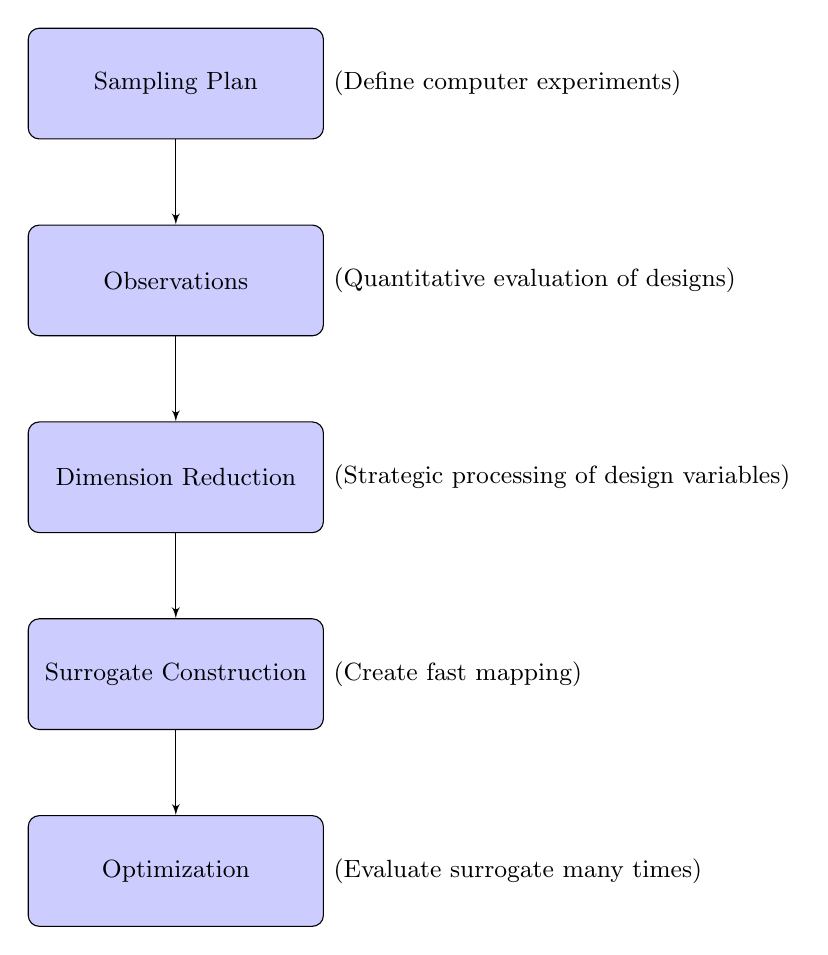
\begin{tikzpicture}[node distance = 2.5cm, auto]
\tikzstyle{every node}=[font=\small]
\node[block, label=right:(Define computer experiments)] (samp_plan) {Sampling Plan};
\node[block, below of= samp_plan, label=right:(Quantitative evaluation of designs)] (obs) {Observations};
\node[block, below of= obs, label=right:(Strategic processing of design variables)](dim_red) {Dimension Reduction};
\node[block, below of= dim_red, label=right:(Create fast mapping)](surr) {Surrogate Construction};
\node[block, below of= surr, label=right:(Evaluate surrogate many times)](opt) {Optimization};
\path [line] (samp_plan.south) -- (obs.north);
\path [line] (obs.south) -- (dim_red.north);
\path [line] (dim_red.south) -- (surr.north);
\path [line] (surr.south) -- (opt.north);
\end{tikzpicture}  
\end{figure}

% Optimized Sampling Plans
\section{Optimized Sampling Plans} \label{sec:sampling_plans}

The following section is concerned with the problem of identifying an optimal set of points at which to build a surrogate model for an expensive computer code when only $N$ evaluations can be afforded. All surrogate models are built around a set of points at which the objective computer code is actually evaluated. Intuitively, the surrogate accuracy is expected to decrease as one moves further away from such points. Consequently, it is important to spread $N$ points as uniformly as possible across the design space. 

\subsection{Morris Algorithm}
\label{subsec:morris_algorithm}

Expensive computer codes generally have many input parameters because they attempt to model some phenomena on a very fine scale as accurately as possible. Of course, when writing such computer codes engineers are not aware which input parameters have the greatest impact on the outputs of interest or else only these parameters would be modeled. Contrarily, engineers typically only know that certain parameters are involved in the pertinent physics in some way but not to what extent. Due to the curse of dimensionality, the less design variables considered in the construction of a surrogate the cheaper the computational cost will be \cite{Forrester}. Consequently, before attempting to construct a surrogate for an expensive computer code it is worth identifying which design variables are most active. After all, if a design variable has a trivial effect on some output of interest then its presence in the surrogate should be minimized, for this is the very purpose of a surrogate model. One method for weeding out unimportant design variables is described by Morris \cite{Morris}, which is summarized in algorithm \ref{code:morris_algorithm}.   

The premise of Morris' algorithm is that if the derivative of some output parameter with respect to a design variable changes significantly throughout the design space then the variable is important. If the output parameter does not change with respect to the design variable then the variable can safely be ignored. To this end, the metric in Eq. \ref{eq:elementary_effect_x} is introduced by Morris to estimate the so-called elementary effect $d_i\left(\textbf{x}\right)$ of design variable $x_i$.
\begin{equation}
\label{eq:elementary_effect_x}
   d_i\left(\textbf{x}\right) = \frac{f\left(x_1,x_2,...,x_{i-1},x_i+\Delta,x_{i+1},....,x_k 										\right) - f\left(\textbf{x}\right)}
   								{\Delta}      
\end{equation}  
In Eq. \ref{eq:elementary_effect_x}, $\Delta$ is a step-length size for the perturbation. For convenience all variables $x_i$ are normalized to unit length and divided into $p$ segments such that $x_i\in\lbrace 0,1/(p-1),2/(p-1),...,1\rbrace$. Choosing a set of $\textbf{x}$ carefully, it is possible to calculate an elementary effect for each of $k$ design variables using only $k+1$ function evaluations. Indeed, as described in \cite{Morris}, a $[k+1]\times [k]$ random orientation matrix $B^*$ can be constructed using the equation,
\begin{equation}
\label{eq:random_orientation}
   \textbf{B}^* = \left(\textbf{1}_{k+1,1}\textbf{x}^* + \frac{\Delta}{2}\left[
                   \left(2\textbf{B} - \textbf{1}_{k+1,k}\right)\textbf{D}^* + 
                    \textbf{1}_{k+1,k}\right]\right)\textbf{P}^*.
\end{equation}            
In Eq. \ref{eq:random_orientation}, $\textbf{1}$ is a matrix of ones with size specified by its subscript and $\textbf{B}$ is a $[k+1]\times [k]$ matrix of zeros and ones with the characteristic that for each column there exists a pair of rows differing in only their $i^{th}$ entry for $i\in\lbrace 1,2,...,k\rbrace$. Also, $\textbf{D}^*$ is a $[k]\times [k]$ diagonal matrix with ones of differing parity uniformly spread, $\textbf{P}^*$ is a $[k]\times [k]$ random permutation matrix, and $\textbf{x}^*$ is a random point chosen in the $p$-level design space. When the rows of $\textbf{B}^*$ are evaluated by the objective function and substituted into Eq. \ref{eq:elementary_effect_x} an elementary effect is calculated for each design variable. 

The more elementary effects that can be calculated for each design variable, the better the estimate as to the effect of each design variable on the objective function. Consequently, $r$ random orientation matrices are typically created to obtain a total of $r$ elementary effects for each design variable. Taking the mean and standard deviation of each variable's $r$ effects can yield insight into the most important variables. Plotting the mean and standard deviation of each variable's effects on a scatter plot, variables that have a negligible effect on the objective function will cluster around the origin. Large fluctuations in standard deviation are indicative of nonlinear and interactive effects \cite{Morris}. 

\begin{algorithm}
\caption{\label{code:morris_algorithm} 
Uses Morris' Algorithm to determine which of a function's design variables induce the most significant effects and interactions.} 
\begin{algorithmic}[1]
\State Initialize zeros matrix $d_{stats}$ of size $[r]\times[k]$
\For {$i=1:r$}
   \State $X\rightarrow$ Create random orientation matrix 
   \Comment{Eq. \ref{eq:random_orientation}} 
   \State $f_{base} = f(X[0,:])$
   \For {$j=1:k$}
      \State $f_{new} = f(X[k,:])$
      \State $l\rightarrow$ Find index of effect being perturbed
      \State $d_{effect}\rightarrow$ Calculate elementary effect \Comment{Eq. \ref{eq:elementary_effect_x}} 
      \State $d_{stats}[i,l] = d_{effect}$
      \State $f_{base} := f_{new}$
   \EndFor
\EndFor
\State Return mean and standard deviation of $d_{stats}$ 
\end{algorithmic}
\end{algorithm}

\subsection{Latin Hypercube Sampling}
\label{subsec:lhs}

One of the major problems with random sampling occurs when a relatively limited sample size is utilized. In this case, subsets of the sample space with high consequence but low probability are likely to be missed \cite{Helton}. In addition, the proximity of sampled values caused by random sampling is inefficient, which often causes slow convergence. In order to resolve such issues \ac{LHS} was conjured. The basis of \ac{LHS} rests upon dividing the normalized space of each design variable into $n$ equally sized bins if $n$ samples are required. As a result, when the $n$ samples are taken it is guaranteed that the entire spectrum of each design variable's space has been visited. Algorithmically an $n$ sample Latin hypercube in $k$ dimensions can be easily calculated, as described in algorithm \ref{code:lhs}.

\begin{algorithm}
\caption{\label{code:lhs} 
Creates a random Latin hypercube consisting of $n$ samples in $k$ dimensions.} 
\begin{algorithmic}[1]
\State Initialize zeros matrix $X$ of size $[n]\times[k]$
\For {$i=1:k$}
   \State $p\rightarrow$ Create random permutation of the set $\lbrace 1,2,...,n\rbrace$ 
   \State $X[:,i] := p[:]$
\EndFor
\State Map each entry of $X$ into hypercube
\State Return $X$ 
\end{algorithmic}
\end{algorithm}

Each row of the output from algorithm \ref{code:lhs} is a sample point normalized to a hypercube. As mentioned previously, when sampling a design space it is important to take sample points uniformly. While \ac{LHS} increases the likelihood of obtaining such a uniform sampling space at random it is actually possible to obtain an optimized sampling space based on the maximin metric \cite{Forrester}.

The maximin metric describe by Morris and Mitchell \cite{Morris_Mitchell} makes use of two notions in an attempt to quantify the uniformity, or 'space-fillingness', of a set of sampling points. In order to describe the notions for each sampling plan it is useful to gather $\lbrace d_1, d_2, ..., d_m\rbrace$ and $\lbrace J_1, J_2, ..., J_m\rbrace$, the unique distances between all points in the plan sorted in ascending order and the number of occurrences of each distance, respectively. In words, the Morris and Mitchell criteria states that an optimized sampling plan will minimize all $J_i$ while maximizing the corresponding $d_i$. More formally, Morris and Mitchell define the maximin sampling plan as one which maximizes $d_1$, and among plans for which this is true, minimizes $J_1$, among plans for which this is true, maximizes $d_2$, and so on \cite{Forrester}. The previous definition can be restated into pseudo-equivalent minimization problem by introducing the parameter $\Phi_q(\textbf{X})$,
\begin{equation}
\label{eq:Phi_q}
   \Phi_q(\textbf{X}) = \left(\sum_{j=1}^m J_j d_j^{-q} \right)^{1/q}
\end{equation}
where $\textbf{X}$ is a sampling plan and $q$ is a control parameter inherent in the minimization problem. 

The minimization of Eq. \ref{eq:Phi_q} and the Morris and Mitchell definition of the maximin sampling plan are generally used in unison to obtain a locally optimal sampling plan since finding the globally optimal plan is computationally infeasible. In this approach a random sampling plan $\textbf{X}_0$ is initially generated using algorithm \ref{code:lhs}. Using a range of $q$ values, usually from one to one-hundred, an optimal latin hypercube plan is found for each value based on the initial sampling plan $\textbf{X}_0$. To obtain an optimized plan for each $q$ algorithms such as simulated annealing \cite{Kirkpatrick} and evolutionary operation \cite{Box} can be used. These algorithms work to minimize Eq. \ref{eq:Phi_q} by comparing an initial sampling plan to perturbed versions, which are obtained by switching pairs of column entries in the output of algorithm \ref{code:lhs}. Once an optimized \ac{LHS} plan is found for each $q$ value, the resulting set of plans are contested directly against each other by explicit application of Morris and Mitchell's maximin definition. The sampling plan satisfying the maximin criteria is the locally optimal sampling plan to be used for proceeding surrogate model construction. Algorithm \ref{code:best_lhs} summarizes the search for a locally optimal \ac{LHS} plan.  

\begin{algorithm}
\caption{\label{code:best_lhs} 
Obtains a locally optimal \ac{LHS} plan using the Morris-Mitchell minimax criteria.} 
\begin{algorithmic}[1]
\State Initialize sampling plan $\textbf{X}_0$ \Comment{Apply algorithm \ref{code:lhs}}
\State $q = \left[1, 2, 5, 10, 20, 50, 100\right]$
\State $\textbf{X}^{cands.} \rightarrow$ Initialize empty array for optimal $\textbf{X}$ candidates
\For {$q_i$ in $q$}
   \State $\textbf{X}_{opt}(q_i)\rightarrow$ Find optimal $\textbf{X}$ for $q_i$ using simulated annealing \Comment{Minimize Eq. \ref{eq:Phi_q}}
   \State Add $\textbf{X}_{opt}(q_i)$ to $\textbf{X}^{cands.}$ 
\EndFor
\State Apply Morris-Mitchell criterion between all $(\textbf{X}^{cands.}_i, \textbf{X}^{cands.}_j)$ to find optimal plan
\end{algorithmic}
\end{algorithm}
  


 


% Kriging
\section{Kriging} \label{sec:kriging}

Write about Kriging!
% Function Decompositions
\section{Function Decompositions} \label{sec:func_decomp}

In order to reduce the dimensionality of some function there must exist a metric to determine the importance of each dimension with respect to the others. It's important to have a framework that isolates the effects of each dimension on the output of the function. The framework chosen to perform dimension reduction is formally known as \ac{HDMR}. In statistics, the \ac{ANOVA} decomposition is a special case of \ac{HDMR} where the Lesbegue measure is used to perform all integrations.

\subsection{Dimension-wise Decompositions} \label{subsec:dim_wise_decomps}

The dimension-wise \ac{HDMR} is algorithmically similar to Gram-Schmidt for matrix orthogonalization in that orthogonal components are systemtically removed to create a linearly independent basis. As in Gram-Schmidt, the essential operator in dimension-wise \ac{HDMR} is the projection operator. Before introducing the projection operator of interest in this thesis, define the $d$-dimensional product measure to be,
\begin{equation} \label{eq:d_dimension_product_measure}
    d\mu\left(\textbf{x}\right) = \prod_{j=1}^{d}
                              d\mu_{j}\left(x_j\right) 
\end{equation}
where $\mu_j$ are probability measures defined over some $\Omega$. Two functions $f,g:\Omega^d \rightarrow \mathbb{R}$ are considered orthogonal with respect to the product measure defined in \ref{eq:d_dimension_product_measure} if the inner product,
\begin{equation} \label{eq:inner_product}
   \left(f,g\right)=\int_{\Omega^d} f(\textbf{x})g(\textbf{x})d\mu(\textbf{x})
\end{equation} 
is equal to zero. To introduce the projection operator $P_\textbf{u}$, the notation used in \cite{Holtz} is adopted. The operator $P_\textbf{u}$ projects from a $d$-dimensional space to a $\vert\textbf{u}\vert$-dimensional space for some set $\textbf{u}\subseteq \mathcal{D}$, where $\mathcal{D}=\lbrace 1,...,d\rbrace$ consists of the set of all coordinate indices in $\textbf{x}$. The projection on to $\textbf{u}$ is given as,
\begin{equation} \label{eq:projection_operator}
    P_\textbf{u}f\left(\textbf{x}_{\textbf{u}}\right) =
     \int_{\Omega^{d-\vert\textbf{u}\vert}} 
      f\left(\textbf{x}\right)d\mu_{\mathcal{D}\setminus\textbf{u}}
       \left(\textbf{x}\right)
\end{equation}
where $\textbf{x}_\textbf{u}$ has length $\vert\textbf{u}\vert$ and consists of the $\textbf{x}$ coordinates specified in $\textbf{u}$. Also, the notation $\mathcal{D}\setminus\textbf{u}$ signifies all the coordinates in $\mathcal{D}$ not contained in $\textbf{u}$. From \ref{eq:projection_operator} it is clear that the projection operator works to integrate out all coordinate indices not contained in $\textbf{u}$ from $f$. For some coordinate indice sets $\textbf{u}$ and $\textbf{v}$, where $\textbf{u}\neq\textbf{v}$, the following orthogonality relation holds,
\begin{equation} \label{eq:orthogonality_relation}
    \left(f_\textbf{u},f_\textbf{v}\right) = 0.
\end{equation}
The notation $f_\textbf{u}$ is used to denote the function of only the coordinate indices contained in $\textbf{u}$. From \ref{eq:orthogonality_relation}, it follows that a function can be written in terms of its $2^d$ orthogonal components,
\begin{equation} \label{eq:hdmr_decomp}
    f\left(\textbf{x}\right) = 
     \sum_{\textbf{u}\subseteq\mathcal{D}}
      f_\textbf{u}\left(\textbf{x}_\textbf{u}\right)
\end{equation}
where the component functions $f_\textbf{u}$ are defined recursively as \cite{Holtz},
\begin{equation} \label{eq:recurvsive_component_def}
    f_\textbf{u}\left(\textbf{x}_\textbf{u}\right) = 
     P_\textbf{u}f\left(\textbf{x}_\textbf{u}\right) -
      \sum_{\textbf{v}\subset\textbf{u}}
       f_\textbf{v}\left(\textbf{x}_\textbf{v}\right).  
\end{equation}
The recursive definition in \ref{eq:recurvsive_component_def} can be written explicitly as,
\begin{equation} \label{eq:explicit_component_def}
    f_\textbf{u}\left(\textbf{x}_\textbf{u}\right) =
     \sum_{\textbf{v}\subseteq\textbf{u}}
      \left(-1\right)^{\vline\textbf{u}\vline-\vline\textbf{v}\vline}
       P_\textbf{v}f\left(\textbf{x}_\textbf{v}\right)    
\end{equation}

For most functions arising in engineering applications, especially if the function is a computer code, the decomposition in \ref{eq:hdmr_decomp} is not possible to obtain because each component function $f_\textbf{u}$ will require a high-dimensional integral to be performed. Of course, this statement assumes a Lebesgue measure in the definition of $d\mu$ in \ref{eq:d_dimension_product_measure}. Alternatively, if a Dirac measure is used then the computationally burdensom integral in \ref{eq:projection_operator} is reduced to a single function evaluation. In this case, the decomposition in \ref{eq:hdmr_decomp} is referred to as an anchored-\ac{ANOVA} decomposition, or CUT-\ac{HDMR} \cite{AHSGC_HighDimensions}.

\subsection{Anchored-ANOVA Decomposition} \label{subsec:anchored_anova}

Using the Dirac measure $\delta(\textbf{x}-\textbf{a})d\textbf{x}$ to evaluate the projection operator at a fixed point $\textbf{a} \in \left[0,1\right]^d$ in the hypercube, equation \ref{eq:projection_operator} becomes,
\begin{equation} \label{eq:projection_operator_dirac}
    P_\textbf{u}f\left(\textbf{x}_\textbf{u}\right) = 
     f\left(\textbf{x}\right)\vert_{\textbf{x}=
      \textbf{a}\setminus\textbf{x}_\textbf{u}}.
\end{equation}
The notation $\textbf{a}\setminus\textbf{x}_\textbf{u}$ is the anchor point $\textbf{a}$ except at the coordinate indices specified in $\textbf{u}$. At the coordinate indices $\textbf{u}$, the anchor point takes upon the corresponding values in $\textbf{x}$. Using the Dirac measure to evaluate the projections comprising \ref{eq:hdmr_decomp}, the objective function is expressed as a linear combination of its values along lines, faces, hyperplanes,..., etc \cite{Holtz}. As mentioned previously, using the Dirac measure to perform the projection operations in \ac{HDMR} results in enormous computational savings since high-dimensional integrals are replaced with single function evaluations.

Given the structure of anchored-\ac{ANOVA}, it is not surprising to learn that there exists a close connection to multivariate Taylor series\cite{HDMR}. This connection provides insight into some of the properties of the anchored-\ac{ANOVA} decomposition. The multivariate Taylor series of $f(\textbf{x})$ about a point $\textbf{\=x}$ can be written as,
\begin{equation} \label{eq:multivariate_Taylor_series}
    f\left(\textbf{x}\right) = 
     f\left(\bar{\textbf{x}}\right) +
      \sum_{i=1}^{d} 
       \frac{\partial f(\textbf{x})}{\partial x_i}\left(x_i - \bar{x}_i\right)
        + \frac{1}{2!}\sum_{i,j=1}^{d}
         \frac{\partial^2 f(\textbf{x})}{\partial x_i\partial x_j}
          \left(x_i - \bar{x}_i\right) \left(x_j - \bar{x}_j\right) + ...
\end{equation}       
As an example, consider what happens if \ref{eq:multivariate_Taylor_series} is evaluated at $\textbf{x} = \textbf{a}\setminus x_i$,
\begin{equation} \label{eq:Taylor_series_ex1}
    f\left(\textbf{x}\right)\vert_{\textbf{x} = \textbf{a}\setminus x_i} = 
     f\left(\bar{\textbf{x}}\right) +
      \frac{\partial f(\textbf{x})}{\partial x_i}\left(x_i - \bar{x}_i\right)
       + \frac{1}{2!} \frac{\partial^2 f(\textbf{x})}{\partial x_i^2}
        \left(x_i - \bar{x}_i\right)^2 + ...
\end{equation}
Since $f_i\left(x_i\right) = f\left(\textbf{x}\right)\vert_{\textbf{x} = \textbf{a}\setminus x_i} - f\left(\bar{\textbf{x}}\right)$, 
\begin{equation} \label{eq:Taylor_series_ex2}
    f_i\left(x_i\right) =
     \frac{\partial f(\textbf{x})}{\partial x_i}\left(x_i - \bar{x}_i\right)
       + \frac{1}{2!} \frac{\partial^2 f(\textbf{x})}{\partial x_i^2}
        \left(x_i - \bar{x}_i\right)^2 + ...      
\end{equation}  
Expression \ref{eq:Taylor_series_ex2} shows that the first-order component functions in anchored-\ac{ANOVA} consist of entire Taylor series expansions. Similarly, second-order component functions will consist of their respective entire Taylor series expansions and so on. Consequently, a truncated anchored-\ac{ANOVA} expansion will always provide a better approximation to a function than a truncated Taylor expansion \cite{HDMR}. 

\subsubsection{Effective Dimensions} \label{subsec:effective_dims}

The ultimate purpose of introducing an expansion such as anchored-\ac{ANOVA} is to truncate it and use the truncated portion as an approximation to the objective function. Of course, evaluation of the truncated anchored-\ac{ANOVA} expansion is expected to be much more computationally efficient than the objective function. When an anchored-\ac{ANOVA} decomposition is truncated, the loss incured becomes the components \ref{eq:recurvsive_component_def} that are not being represented. Of course, in practical construction the components not represented are calculated to contribute relatively trivially. Two notions exist for classifying the dimension of a truncated anchored-\ac{ANOVA} decomposition. Both notions depend on $\hat{\sigma}(f)$, which is the sum of the absolute values of the integrals of all anchored-\ac{ANOVA} terms \cite{Holtz}
\begin{equation} \label{eq:sum_all_integrated_components}
    \hat{\sigma}\left(f\right) = 
     \sum_{\begin{subarray}
     \textbf{u} \subseteq \mathcal{D} \\
     \textbf{u} \neq \emptyset
     \end{subarray}}
      \vert If_\textbf{u} \vert \approx
       \sum_{\begin{subarray}
       \textbf{u} \subseteq \mathcal{D} \\
       \textbf{u} \neq \emptyset
       \end{subarray}}
        \vert q_\textbf{u} \vert .
\end{equation}
The notation $I\cdot$ represents an exact integral but, in practice the integral will be evaluated using some multivariate quadrature scheme and so the exact integral's approximation is denoted by $q_\textbf{u} \approx If_\textbf{u}$. For some user-defined threshold $\alpha \in \left[0,1\right]$ the truncation and superposition dimensions of a truncated anchored-\ac{ANOVA} expansion can be defined. The truncation dimension attempts to quantify the importance of a certain number of dimensions $d_t$. Mathematically, the truncation dimension is the smallest integer $d_t$ such that,
\begin{equation} \label{eq:trunc_dimension}
    \sum_{
     \begin{subarray}{c}
     \textbf{u} \subseteq \lbrace1,...,d_t\rbrace \\
     \textbf{u} \neq \emptyset
     \end{subarray}
    } 
     \vert q_\textbf{u} \vert \geq \alpha \hat{\sigma}(f). \nonumber
\end{equation}
Contrastingly, the superposition dimension attempts to quantify the order of important dimensions $d_s$. Mathematically, the superposition dimension is the smallest dimension $d_s$ such that,
\begin{equation} \label{eq:sup_dimension}
    \sum_{
     \begin{subarray}{c}
     \vert\textbf{u}\vert \leq d_s \\
     \textbf{u} \neq \emptyset
     \end{subarray}
    } 
     \vert q_\textbf{u} \vert \geq \alpha \hat{\sigma}(f). \nonumber
\end{equation}
       
Both definitions for the effective definition of a truncated anchored-\ac{ANOVA} expansion can be directly related to the exact integral of the objective function $If$. Specifically, for the truncation dimension the following relation holds \cite{Holtz},
\begin{equation} \label{eq:trunc_dim_error}
    \vert If -  
     \sum_{\textbf{u} \subseteq \lbrace 1,...,d_t\rbrace}
      If_\textbf{u} 
    \vert \leq \left(1-\alpha\right) \hat{\sigma}\left(f\right).
\end{equation}
Similarly, for the superposition dimension the following inequality holds,
\begin{equation} \label{eq:superpos_dim_error}
    \vert If -  
     \sum_{\vert \textbf{u} \vert \leq d_s}
      If_\textbf{u} 
    \vert \leq \left(1-\alpha\right) \hat{\sigma}\left(f\right).
\end{equation}
Ineqalities \ref{eq:trunc_dim_error} and \ref{eq:superpos_dim_error} suggest that if all the anchored-\ac{ANOVA} terms are used then the exact integral of the objective function can be reproduced. However, in general the set of effective dimensions as determined by anchored-\ac{ANOVA} will not be equal to the set determined by a classic \ac{ANOVA} decomposition. The choice of the anchor point $\textbf{a}$ has a direct influence on the accuracy and truncation dimension of the anchored-\ac{ANOVA} expansion \cite{Hesthaven_AnchorPoint}. In \cite{Hesthaven_AnchorPoint} the authors argue that choosing the anchor point to be the centroid of the parameter space is an excellent choice for most applications. As such, in this thesis the anchor point is always chosen to be the centroid of the working parameter space $\Omega^d$.    

% Smolyak Sparse Grids
\section{Smolyak Sparse Grids} \label{sec:smolyak_sg}

In order to create a reduced-order model for some objective function the anchored-\ac{ANOVA} decomposition plays a crucial role but more is needed \cite{Hesthaven_ANOVA}. Recall that the primary purpose for constructing a reduced-order model is to replace the presumably computationally intensive objective function with something that is trivial to evaluate. Consequently, in evaluating the anchored-\ac{ANOVA} decomposition at some point $\textbf{x}$ the projections in  \ref{eq:projection_operator_dirac} must be trivial to evaluate as well. As it stands, evaluating the anchored-\ac{ANOVA} decomposition for some objective function is significantly more expensive than simply evaluating the function itself. To resolve this issue, a Smolyak sparse grid interpolant is created for each projection. While creating each such interpolant incurs some initial overhead, the payoff is the desired reduced order model. 

\subsection{Motivation} \label{subsec:motivation}

To describe multivariate function interpolation based on Smolyak sparse grids it makes sense to speak in the context of quadrature since a quadrature rule consists of interpolating a function using polynomials and then integrating the polynomials exactly. For the moment consider some smooth 1D function $f(x)$. The function $f(x)$ can be approximated arbitrarily well through the summation,
\begin{equation} \label{eq:1D_interp}
   f(x) \approx \sum_{i=1}^{P} f(x_i)C_i(x)
\end{equation}
where $C_i(x)$ are cardinal functions of degree $P$ with the property that $C_i(x_j)=\delta_{ij}$, $\delta_{ij}$ being the Kronecker $\delta$-function \cite{Boyd}. By the Weierstrass approximation theorem, smooth functions can be uniformly approximated as closely as desired by polynomial functions \cite{TrefethenApprox}. At the collocation points, or abscissas, in \ref{eq:1D_interp} the function $f(x)$ is interpolated exactly at $x_i$. The function $f(x)$ is comprised of various constant, linear, quadratic, cubic,..., etc terms and so exact integration of $f(x)$ amounts to integrating its monomial constituents.  

Suppose that instead of interpolating a 1D function, a multivariate function of $d$ dimensions is to be interpolated. The naive approach to multivariate interpolation is to take a Cartesian product of 1D rules, such as in \ref{eq:1D_interp}, $d$ times. Consequently, the product grid will contain $P^d$ points, each of which requires a unique function evaluation. Such exponential growth is coined the "curse of dimensionality" \cite{LeMaitreKnio}. As a rule of thumb, exact integration of a monomial constituent comes at the cost of a single function evaluation \cite{Burkardt_SCALA2013}. Considering the space of $d$-dimensional, $P$-degree polynomials has some,
\begin{equation} \label{eq:polynomial_space}
    \binom{P+d}{d} \approx \frac{d^P}{P!} 
\end{equation} 
dimensions, for high dimensional problems the full Cartesian product approach integrates a superfluous number of monomials. Russian mathematician Sergei Smolyak was one of the first to realize the potential computational savings in his paper \cite{SmolyakOriginal}.

\subsection{Algorithm Mechanics} \label{subsec:algorithm_mechanics}

A Smolyak sparse grid is the set of collocation points used to build an interpolant for some multivariate objective function while the Smolyak algorithm is the whole procedure of building the interpolant. To begin, the Smolyak algorithm will be stated and pertinent notation will be introduced. Since indice tracking comprises the brunt of understanding the Smolyak algorithm, it is crucial to choose a clear notation. Consequently, the notation used here closely follows that of \cite{NovakRitter}.

Slightly generalizing \ref{eq:1D_interp}, for the case of some smooth 1D function $f$, let $U^i$ be the interpolant of $f$ comprised of $m_i$ collocation points.
\begin{equation} \label{eq:1D_interp2}
    U^i = \sum_{j=1}^{m_i} 
     f\left(x_j^i\right) a_j^i
\end{equation}  
In \ref{eq:1D_interp2}, $i \in \mathbb{N}$, and $a_j^i \in C(\left[-1,1\right])$ are basis functions imposing the demand that $U^i$ exactly be able to reproduce $f$ at the collocation points $x_j^i$. The notation $x_j^i \in \left[-1,1\right]$ refers to the $j^{th}$ collocation point of $m_i$ total points. Restricting the domain of the collocation points to $\left[-1,1\right]$ does not impose any limitations on being able to interpolate $f$ arbitrarily well since $\left[-1,1\right]$ can always be mapped to the parameter space of $f$.

To generalize from 1D interpolation to multivariate interpolation 1D interpolation formulas, such as the one in \ref{eq:1D_interp2}, are combined using tensor products.
\begin{equation} \label{eq:muitivariate_interp_fulltp}
    \left(U^{i_1} \otimes\cdots\otimes U^{i_d}\right)\left(f\right) = 
     \sum_{j_1=1}^{m_{i_1}} \cdots
      \sum_{j_d=1}^{m_{i_d}} f\left(
       x_{j_1}^{i_1},\cdots,x_{j_d}^{i_d}\right)\cdot
        \left(a_{j_1}^{i_1}\otimes\cdots\otimes a_{j_d}^{i_d}\right)
\end{equation}   
Tensor products are a mathematical convenience used to represent all combinations of some entity, in this case $U^i$. The scheme in \ref{eq:muitivariate_interp_fulltp} suffers from the, "curse of dimensionality" since a total of,
\begin{equation}
    \prod_{k=1}^d m_{i_k}
\end{equation}     
function evaluations are needed to form the interpolant. The Smolyak algorithm is based on \ref{eq:muitivariate_interp_fulltp}, the only difference being not all the tensor products are used. In explicit form, the Smolyak formula for approximating the left-hand side of \ref{eq:muitivariate_interp_fulltp} is given as \cite{NovakRitter},
\begin{equation} \label{eq:Smolyak_formula1}
    A\left(q,d\right) = 
     \sum_{q-d+1\leq \vert \textbf{i}\vert\leq q}
      \left(-1\right)^{q-\vert\textbf{i}\vert}
       \binom{d-1}{q-\vert\textbf{i}\vert}
        \left(U^{i_1} \otimes\cdots\otimes U^{i_d}\right).
\end{equation}
Each entry $i_k$ in the vector $\textbf{i} \in \mathbb{N}^d$ contains the indice corresponding to the level of interpolation in dimension $k$. The more collocation points being utilized, the higher the level of interpolation since the interpolant becomes increasingly accurate. The magnitude of $\textbf{i}$ is $\vert\textbf{i}\vert = \vert i_1 +\cdots+ i_d\vert$. Since each $i_d \geq 1$, the variable $q \geq d$. The variable $q$ essentially keeps track of the level of interpolation of the Smolyak algorithm. As $q$ is increased, more tensor product combinations are allowed. From \ref{eq:Smolyak_formula1} it is clear that the Smolyak algorithm is able to reduce the total number of tensor product components by limiting the entries of $\textbf{i}$. Note, when performing analysis using the Smolyak algorithm the "interpolation level" typically refers to $q-d$ in order to ground the analysis at an interpolation level of zero.

The Smolyak formula in \ref{eq:Smolyak_formula1} can be rewritten in several ways, all of which use the idea of the incremental interpolant $\Delta^i$ defined as,
\begin{eqnarray} \label{eq:incremental_interpolant}
    U^0 &=& 0 \nonumber \\
    \Delta^i &=& U^i - U^{i-1}
\end{eqnarray}
The incremental interpolant operator is simply the difference between interpolants at two successive levels. Using the notion of the incremental interpolant, the Smolyak formula can be rewritten as,
\begin{equation} \label{eq:Smolyak_formula2}
    A\left(q,d\right) =
     \sum_{\vert\textbf{i}\vert\leq q}
      \left(\Delta^{i_1}\otimes\cdots\otimes\Delta^{i_d}\right)
\end{equation}   
At first sight, \ref{eq:Smolyak_formula1} and \ref{eq:Smolyak_formula2} seem inefficient since neither exposes the recursiveness inherent in the Smolyak formula. In other words, when moving from index $q$ to $q+1$ the work done to get to level $q$ is not lost. Rewriting the Smolyak formula in a recursive fashion is advantageous for implementation on a computer.
\begin{eqnarray}
\label{eq:Smolyak_formula3a}
    A(q,d) &=& A(q-1,d) + \Delta A(q,d) \\
\label{eq:Smolyak_formula3b}
    \Delta A(q,d) &=& \sum_{\vert\textbf{i}\vert = q}
     \left(\Delta^{i_1}\otimes\cdots\otimes\Delta^{i_d}\right)
\end{eqnarray}
While the Smolyak algorithm representation in \ref{eq:Smolyak_formula3a} has the advantage of being represented recursively, it does not provide any type of indicator for when the Smolyak sparse grid should be refined. Collocation points should be added to a Smolyak sparse grid until the resulting interpolant is able to reproduce the objective function to some user-defined threshold. The authors in \cite{AHSGC} are able to rewrite \ref{eq:Smolyak_formula3b} in terms of what's referred to as a hierarchical surplus, 
\begin{equation} \label{eq:hierarchical_surplus}
    \Delta A(q,d) = \sum_{\vert\textbf{i}\vert=q}
     \left(f(x_{j_1}^{i_1},...,x_{j_d}^{i_d}) - 
      A(q-1,d)(x_{j_1}^{i_1},...,x_{j_d}^{i_d})\right)\cdot
       \left(a_{j_1}^{i_1}\otimes\cdots\otimes a_{j_d}^{i_d}\right)
\end{equation}
which appears as the first term in the summation as the difference between the function value at the point $(x_{j_1}^{i_1},...,x_{j_d}^{i_d})$ and the Smolyak $q-1$ level interpolant value at the same point. Level $q$ of the Smolyak algorithm generally contains all the points comprising level $q-1$ plus some new collocation points. Consequently, the level $q$ Smolyak interpolant is expected to exactly evaluate any collocation points born in previous levels. The summation in \ref{eq:hierarchical_surplus} is taken over all the new points in level $q$ that have not appeared in level $q-1$ since the hierarchical surplus for these will be identically equal to zero. The hierarchical surpluses provide an indicator for how well the Smolyak algorithm is interpolating some objective function. If the hierarchical surpluses are decreasing with each successive level then the Smolyak algorithm is converging.

Following the notation in \cite{NovakRitter}, let $X^i=\lbrace x_1^i,...,x_{m_i}^i\rbrace$ be the collocation points comprising $U^i$. From \ref{eq:Smolyak_formula1}, the total number of collocation points in a Smolyak sparse grid can be written as,
\begin{equation} \label{eq:numer_points_in_smolyak}
    H(q,d) = \bigcup_{q-d+1\leq\vert\textbf{i}\vert\leq q}
     \left(X^{i_1}\times\cdots\times X^{i_d}\right).
\end{equation}     

\subsection{Basis and Collocation Points} \label{subsec:basis_and_points}

The exactness of the Smolyak algorithm is decided mainly by the choice of collocation points $x_{j_k}^{i_k}$ used to build $H(q,d)$. The basis functions $a_{j_k}^{i_k}$ work to weave the collocation points together. Gaussian quadrature is a favorite of many since with only $n+1$ collocation points, all polynomials of degree $2n+1$ or less can be integrated exactly \cite{NumAnyHenrici}. However, collocation points derived from Gaussian quadrature schemes are not nested in that $X^i \not\subset X^{i+1}$. Nestedness in the choice of collocation points is an essential feature for reducing the computational expense of applying the Smolyak algorithm. If nested collocation points are chosen for each $X^{i_k}$ then the Smolyak sparse grid will also be nested such that $H(q-1,d)\subset H(q,d)$ \cite{NovakRitter}. Consequently, when improving the Smolyak interpolant from level $q-1$ to level $q$ one will only have to evaluate the objective function at the points that are unique to $X^i$, which are given as $X_{\Delta}^{i} = X^i \setminus X^{i-1}$ \cite{AHSGC}.  The set of new points in level $q$ of a Smolyak sparse grid are given as,
\begin{equation} \label{eq:unique_points_ssg}
    \Delta H(q,d) = \bigcup_{\vert\textbf{i}\vert = q}
     X_{\Delta}^{i_1} \times\cdots\times X_{\Delta}^{i_d}.
\end{equation}   

A viable alternative to Gaussian quadrature collocation points for the Smolyak algorithm is to use Clenshaw-Curtis collocation points, which consist of the extrema of Chebyshev polynomials. While $n+1$ Clenshaw-Curtis abscissas can only exactly integrate polynomials of degree $n$, they have the advantage of being nested. Accuracy is sacrificed for nestedness in the Smolyak algorithm, at least in theory. In practice it has been shown that for most functions Clenshaw-Curtis quadrature performs almost on par to Gaussian quadrature \cite{TrefethenQuadrature}. In other words, the double accuracy of Gaussian quadrature is rarely realized. For some level $i$ the Clenshaw-Curtis collocation points are given by,
\begin{equation} \label{eq:cc_points}
    x_{j}^{i} = \left\{
     \begin{array}{cr}
       \cos\frac{\pi(j-1)}{m_i-1}   & j=1,...,m_i \text{ if } i>1 \\
       0   &  j=1 \text{ if } i=1
     \end{array}
   \right.
\end{equation}
In order for the level $i$ Clenshaw-Curtis abscissas to contain the level $i-1$    abscissas, a total of $2^{i-1}$ new points must be added. Consequently, the total number of abscissas appearing in the level $i$ Clenshaw-Curtis scheme is given as,
\begin{equation} \label{eq:cc_numpoints}
    m_i = \left\{
     \begin{array}{cr}
      2^{i-1}+1   & i>1 \\
      1   & i=1
     \end{array}
    \right.
\end{equation}

Another alternative to the Gaussian and Clenshaw-Curtis abscissas is Gauss-Patterson. The Gauss-Patterson set of collocation points are nested and provide  a polynomial exactness of $(3n-1)/2$ with $n$ points, which is right in between the exactness of Clenshaw-Curtis and Gaussian sets. Obtaining the Gauss-Patterson abscissas involves a rather convoluted, iterative process and so the reader is referred to \cite{GaussPatterson} to review the methodology and obtain tables of the actual points. The growth rule for Gauss-Patterson goes as $2^i-1$, which is some factor of two greater than the growth rule for Clenshaw-Curtis. In \cite{HesthavenGaussPatt}, the authors conclude the Gauss-Patterson collocation points are competitive with Clenshaw-Curtis when comparing the cost and accuracy of computing quadratures using the same number of function evaluations.       

To weave together the collocation points forming a Smolyak sparse grid, some type of basis function $a_{j}^i$ is needed, as defined in \ref{eq:1D_interp2}. Although the basis functions will be applied to multi-dimensional interpolation, the Smolyak algorithm conveniently scales 1D basis functions to multiple dimensions through the use of tensor products. One basis commonly used  in adaptive sparse grids is the linear hat basis function \cite{Agarwal}. For the scheme in \ref{eq:cc_numpoints} the linear hat functions are given as, 
\begin{eqnarray} \label{eq:linear_hat_basis}
    a_{1}^{1} &=& 1 \text{ for } i=1, \\
    a_{j}^{i} &=& \left\{
     \begin{array}{cc}
      1-(m_i-1)\vert x-x_j^i\vert   & \text{ if }
      \vert x-x_j^i\vert < 1/(m_i-1) \\
       0   & \text{ else } \nonumber
     \end{array}
    \right.
\end{eqnarray}
for $i>1$ and $j=1,...,m_i$. While the linear hat functions have the advantage of local support they are limited to relatively slow convergence due to their lack of curvature. Offering faster error decay are the global Lagrange characteristic polynomials, 
\begin{equation} \label{eq:lagrange_basis}
    a_j^i = \left\{
     \begin{array}{cc}
      1   & \text{ if } i=1 \\
      \displaystyle \prod_{\begin{subarray}{l}
              k=1 \\
              k \neq j
             \end{subarray}}^{m_i}
       \frac{x-x_k^i}{x_j^i-x_k^i}   & j=1,...,m_i \text{ for } i>1    
     \end{array}
    \right.
\end{equation}  
However, the Lagrange characteristic polynomials are plagued by the fact that each evaluation of \ref{eq:1D_interp2} requires $\mathcal{O}(m_i^2)$ operations and  often the computation is numerically unstable \cite{BaryCentIntrp}. To remedy these concerns, the barycentric form of Lagrange characteristic polynomials is used to form a basis. The barycentric Lagrange basis is given as,
\begin{equation} \label{eq:barycentric_basis}
    a_j^i = \left\{
     \begin{array}{cc}
      1   & \text{ if } i=1 \\
      \displaystyle \frac{\frac{w_j^i}{x-x_j^i} }
       {\sum_{j=0}^{m_i} 
        \frac{w_j^i}{x-x_j^i}}   & j=1,...,m_i \text{ for } i>1
     \end{array}
    \right.
\end{equation} 
where $w_j^i$ are barycentric weights defined by,
\begin{equation} \label{eq:barycentric_weights}
    w_j^i = \frac{1}
     {\displaystyle \prod_{k \neq j}\left(x_j^i - x_k^i\right)}
      \hspace{1 cm} j=1,...,m_i.
\end{equation}
For special collocation sets, such as Clenshaw-Curtis in \ref{eq:cc_points}, explicit forms exist for the barycentric weights. Generally, forming the weights is an $\mathcal{O}(m_i^2)$ operation and then evaluation of an interpolant based on the barycentric Lagrange basis is only a $\mathcal{O}(m_i)$ operation \cite{BaryCentIntrp}. With an explicit form in hand, evaluation of the barycentric Lagrange basis is significantly cheaper than the Lagrange basis. For the Clenshaw-Curtis collocation points in \ref{eq:cc_points}, the barycentric weights are given by \cite{ChebyType2},
\begin{equation} \label{eq:barycentric_weights4_cc}
    w_j^i = (-1)^{j+1}\delta_j^i \hspace{1 cm}
     \delta_j^i = \left\{
                   \begin{array}{cc}
                    .5   & j=1 \text{ or } j=m_i \\
                    1   & \text{ else }  
				   \end{array}
				  \right. .                   
\end{equation}      
From \ref{eq:barycentric_basis}, an apparent problem exists if the barycentric basis is to be evaluated at a collocation point. As \cite{BaryCentIntrp} explains, the problem can be circumvented by simply perturbing the value of $x$ by an $\epsilon$ on the order of machine precision. In this case, the numerator and denominator in \ref{eq:barycentric_basis} will effectively cancel each other such that $a_j^i=1$. The barycentric Lagrange basis is therefore numerically stable.  

\subsection{Exactness and Error Bounds} \label{subsec:exactness_error}

The exactness of the Smolyak algorithm is determined by the space of polynomials the algorithm is exact on. Since the 1D interpolation rules, on which the Smolyak algorithm is based on, can exactly interpolate certain polynomials it is not presumptuous to expect the Smolyak algorithm to exactly interpolate certain polynomial spaces. Using the collocation set in \ref{eq:cc_numpoints} and \ref{eq:cc_points} the Smolyak interpolant $A(q,d)$ is exact on \cite{NovakRitter},
\begin{equation} \label{eq:polynomial_exactness}
    \sum_{\vert\textbf{i}\vert = q}
     \mathbb{P}(m_{i_1}-1,1)\otimes\cdots\otimes
      \mathbb{P}(m_{i_d}-1,1)
\end{equation} 
where $\mathbb{P}(k,d)$ is the space of all polynomials in $d$ dimensions of total degree no greater than $k$. From \ref{eq:polynomial_exactness} it follows that the Smolyak interpolant for $q=d+P$ is exact for all polynomials of degree $P$. In other words, the effects of any monomials containing $x^l$ for $l\leq P$ will be captured by the Smolyak algorithm. Recall from \ref{eq:polynomial_space} that the degrees of freedom of $\mathbb{P}(P,d)$ goes as $d^P/P!$. Any method aiming to reproduce $\mathbb{P}$ requires at least this many function evaluations. Since the number of collocation points in a Smolyak grid for $A(d+P,d)$ goes as $2^{P}d^{P}/P!$ the dependence on dimension is said to be optimal \cite{NovakRitter}. However, the asymptotic growth of points also indicates that the Smolyak algorithm requires still excessive function evaluations to achieve polynomial exactness.     

Since the Smolyak algorithm is constructed using one-dimensional interpolation formulas, which all have error bounds, it is also possible to derive error bounds for a Smolyak interpolant $A(q=d+P,d)$. While the reader is instructed to consult \cite{NovakRitter} for a detailed derivation of the error bounds, they will nevertheless be stated here. Consider some $d$-variable function $f$ with continuous derivatives of order $P$ in each variable. The error in using a Smolyak interpolant to approximate $f$ can be given as,
\begin{equation} \label{eq:smolyak_error}
    \Vert f-A(d+P,d)(f)\Vert_{\infty} \leq 
     c_{d,P} M^{-P} (\log M)^{(P+2)(d-1)+1}
\end{equation}
where $M$ is the total number of knots used by $A(d+P,d)$ and $c_{d,P}$ is a constant depending on both $d$ and $P$. From \ref{eq:smolyak_error}, the error in the Smolyak interpolant heavily depends on the smoothness of the function being interpolated and on the total number of collocation points used to form the interpolant.       

\subsection{Computer Implementation} \label{subsec:smolyak_implementation}

To implement Smolyak's algorithm on a computer equations \ref{eq:Smolyak_formula3a} and \ref{eq:hierarchical_surplus} should be utilized since together they provide a recursive definition. Much of the implementation efforts are concerned with indice book keeping. Although the pseudocode for Smolyak's algorithm used in this thesis is provided here, the reader is directed to \cite{Klimke_Wohlmuth} for more elaborate details. Efficiency of the algorithm can be increased by pre-calculating the desired abscissas as in \ref{eq:cc_points}, the number of abscissas at a given level as in \ref{eq:cc_numpoints}, and corresponding barycentric weights as in \ref{eq:barycentric_weights4_cc}. A data structure for quick retrieval of the desired values is also necessary. Abscissa information is constantly being reused in Smolyak's algorithm and so it is inefficient to have to recalculate values each time.   
\begin{algorithm}
\caption{\label{code:smolyak_algorithm} Smolyak's algorithm for creating an interpolant for a function $f$ of $d$ dimensions. The algorithm will exit if the maximum Smolyak level is reached or if one of the convergence criteria is met.}  
\begin{algorithmic}[1]
\State {Create data structure that stores indice coordinates and hierarchical surplus.}
\For{$q=d,\text{maximum level}$}
   \For{$(i_1,...,i_d)$ in enumerations of $i_1+...+i_d=q$}
   \Comment{See Alg. \ref{code:enumeration1}}
      \For{$(j_1,...,j_d)$ in enumerations of $(i_1,...,i_d)$}
      \Comment{See Alg. \ref{code:enumeration2}}   
         \State {Turn each $(j_1,...,j_d)$ into a knot.} 
         \State {Categorize as either processed or unprocessed knot.}    
      \EndFor
      \State Evaluate $f(\text{unprocessed knots})$.
      \State Calculate hierarchical surplus at unprocessed knots. 
      \Comment{Eq. \ref{eq:hierarchical_surplus}}
      \State Archive newly processed knots.
   \EndFor
   \State Check for convergence.
\EndFor 
\end{algorithmic}
\end{algorithm}

The pseudocode for Smolyak's algorithm in algorithm \ref{code:smolyak_algorithm} will now be discussed in some detail. To initialize the algorithm a data structure must be created to store all information for each index in the sparse grid. For level $q$ of the Smolyak algorithm the summation in \ref{eq:Smolyak_formula3a} is over all sets $(i_1,i_2,...,i_d)$ such that $i_1 + i_2 + ... + i_d = q$. Each such set corresponds to a knot $(x^{i_1}_{j_{i_1}}, ..., x^{i_d}_{j_{i_d}})$ in the random space defined by the hypercube $\left[-1,1\right]^d$. The knot, function value at the knot, and the corresponding hierarchical surplus should all be stored in the data structure. 

The first loop in the pseudocode tells the code to keep increasing the interpolation level in the Smolyak algorithm until some maximum level is reached, which is specified by the user. The purpose of this loop is to make sure the algorithm ends eventually. Of course, other convergence criteria are in place in hope that the algorithm terminates long before the maximum level is reached. The second loop goes through all the enumerations of $(i_1,i_2,...,i_d)$ such that $i_1 + i_2 + ... + i_d = q$. The algorithm for producing such enumerations is provided in algorithm \ref{code:enumeration1}. The third loop takes each enumeration and again enumerates over each index to obtain each component in the tensor product appearing in the Smolyak formulation. An algorithm to execute this enumeration is provided in algorithm \ref{code:enumeration2}.

In the main body of the pseudocode each output from algorithm \ref{code:enumeration2} is first converted to a knot $(x^{i_1}_{j_{i_1}}, ..., x^{i_d}_{j_{i_d}})$. Each potential knot must then be sorted into one of two categories. The motivation for the two categories arises from the fact that the same knot may be expressed in several ways. Since each knot corresponds to a function value and hierarchical surplus, significant computational savings can be incurred by not reevaluating the objective function at the same knots. Consequently, each potential knot is binned into either a category of knots that have already been evaluated at $f$ or a category of unevaluated knots.

Once all components in the tensor product for a given $(i_1,i_2,...,i_d)$ have been converted and sorted, the unevaluated knots are processed. In this step of the algorithm the previously unevaluated knots should be evaluated at $f$ in parallel if possible since each evaluation is completely independent. The resulting functions values should then be used to compute the hierarchical surplus in \ref{eq:hierarchical_surplus} for each knot. Once the function value and hierarchical surplus is available for each new knot the results should be archived in the indice data structure.     

Finally, once the second loop is complete, the level of the Smolyak interpolant has been effectively increased and it's time to check whether additional levels are required based on user-defined convergence criteria. Perhaps the best indicator of a Smolyak interpolant's convergence is the maximum hierarchical surplus calculated for all newly processed knots at the current interpolation level. The hierarchical surplus is a measure of how well the interpolant is able to match the objective function and therefore, if the hierarchical surpluses being calculated are decreasing with each level the interpolant is converging. An additional convergence criteria includes comparison of the relative change in computed mean and variance between two successive interpolation levels. For this thesis, the Smolyak algorithm is terminated only after the maximum hierarchical surplus is below a certain threshold, the relative change in interpolant mean is below a threshold, and the relative change in variance does not exceed a threshold. 
% Combining Decomposition and Interpolation
\section{Combining Decomposition and Smolyak's Algorithm} \label{sec:decomp_and_interp}

As hinted at in the beginning of chapter \ref{chap:rom}, the Smolyak algorithm combines with the anchored-\ac{ANOVA} decomposition to create a reduced order model for any well behaving computer code. To see how the Smolyak algorithm fits into the functional decomposition described in this chapter, begin by substituting \ref{eq:explicit_component_def} into \ref{eq:hdmr_decomp} to get,
\begin{equation} \label{eq:decomp_smol1}
   f(\textbf{x}) = 
    \sum_{\textbf{u}\subseteq\mathcal{D}}
     \sum_{\textbf{v}\subseteq\textbf{u}} 
      (-1)^{\vert\textbf{u}\vert - \vert\textbf{v}\vert}
       P_{\textbf{v}} f(\textbf{x}_{\textbf{v}}).
\end{equation} 
Now, insert the Dirac projection operator from \ref{eq:projection_operator_dirac} into \ref{eq:decomp_smol1} to arrive at,  
\begin{equation} \label{eq:decomp_smol2}
   f(\textbf{x}) = 
    \sum_{\textbf{u}\subseteq\mathcal{D}}
     \sum_{\textbf{v}\subseteq\textbf{u}} 
      (-1)^{\vert\textbf{u}\vert - \vert\textbf{v}\vert}
       f(\textbf{x})\vert_{  
        \textbf{x}=\textbf{a}\setminus\textbf{x}_{\textbf{v}} }.   
\end{equation}
To create a reduced order model the set $\mathcal{D}$ is ultimately shrunk to only contain a subset of all the variables of $f$ but this is discussed later. The important aspect of \ref{eq:decomp_smol2} to realize is that in order to evaluate $ f(\textbf{x}) \vert_{\textbf{x} = \textbf{a} \setminus \textbf{x}_{\textbf{v}}}$ evaluation of the expensive computer code $f(\textbf{x})$ is required. Consequently, the desireable property of reduced order models, that of rapid evaluation, is not achieved in \ref{eq:decomp_smol2}. The remedy is to approximate each $ f(\textbf{x}) \vert_{\textbf{x} = \textbf{a} \setminus \textbf{x}_{\textbf{v}}}$ using Smolyak interpolants. Substituting \ref{eq:Smolyak_formula2} into \ref{eq:decomp_smol2}, the formulation for creating a reduced order model of $f$ is complete. 
\begin{equation} \label{eq:decomp_smol3}
   f(\textbf{x}) = 
    \sum_{\textbf{u}\subseteq\mathcal{D}}
     \sum_{\textbf{v}\subseteq\textbf{u}} 
      (-1)^{\vert\textbf{u}\vert - \vert\textbf{v}\vert}
       \sum_{\vert\textbf{i}\vert\leq q}\left(
        \Delta^{i_1}\otimes\cdots\otimes\Delta^{i_{\vert\textbf{v}\vert}}
         \right)  
\end{equation}
While there is initial overhead to create an interpolant for each component in \ref{eq:decomp_smol2} the result is quick evaluation of the reduced order model. Details regarding the implementation and application of \ref{eq:decomp_smol3} will be discussed in the proceeding sections.               
 
\subsection{Implementation Details} \label{subsec:implement_details}
%Discuss combinatorics routines needed(2, list in appendix), algorithm, sampling, identify important dimensions, when to truncate decomposition. Low order smolyak grids needed is has been shown. First order should be good most of time...especially in nuclear applications where adjoints have been so successful.

\subsubsection{Combinatorics Routines} \label{subsubsec:combinatorics_routines}

In order to implement \ref{eq:decomp_smol3} on a computer several enumeration routines need to be available. Unfortunately, these routines are not available in most numerical math libraries containing combinatorics routines. The first routine of interest solves the problem of how to enumerate all the ways $d$ positive integers can be summed to equal another integer. In other words, what are all the sets $\left\{i_1,...,i_d\right\}$ such that $i_1 + i_2 + ... + i_d = q$? This problem inserts itself in \ref{eq:decomp_smol3} in the summation index for Smolyak interpolation. As the Smolyak interpolant becomes refined from level to level---$q$ is increased by one in each refinement---the Smolyak algorithm must newly account for all $\textbf{i}$ such that $\vert\textbf{i}\vert=q$. The following enumeration algorithm, a slight modification of the original algorithm found in \cite{Holtz}, finds all the desired indice sets:        
\begin{program} 
\begin{code}
# Initialize
p = 0
m = q - d + 1 
k = [0,1,...,1]   # vector of length d
kh = [m,m,...,m]  # vector of length d

# Begin algorithm...
repeat until k = [0,...,0]:
   k(p) = k(p) + 1
   if k(p) > kh(p):
      if p == d:
         All indices enumerated!
      else:
         k(p) = 1
         p = p + 1
   else:
      for j in range(p):
         kh(j) = kh(p) - k(p) + 1
      k(0) = kh(0)
      p = 1
      Return valid index set k!
\end{code}
\caption{\label{code:enumeration1} 
For postitive integers $d$ and $q$ this code outputs all sets $\left\{i_1,i_2,...,i_d\right\}$ such that $i_1+i_2+...+i_d=q$.}  
\end{program}

With all the index sets for some Smolyak level $q$ available through the code segment in \ref{code:enumeration1}, the tensor product appearing in \ref{eq:Smolyak_formula2} can be evaluated with the aid of an additional enumeration routine. Each indice in an index set $\left\{i_1+i_2+...+i_d\right\}$ corresponds to certain number of knots, which for example, is given by \ref{eq:cc_numpoints} for Clenshaw-Curtis. All the components in the tensor product can be given by the following enumeration algorithm, which is based on the algorithm in \cite{Holtz}. Input to the algorithm in code \ref{code:enumeration2} should be based on output from code \ref{code:enumeration1}. Specifically for some index set $\left\{i_1,i_2,...,i_d\right\}$ returned by code \ref{code:enumeration1}, each indice should be converted to a corresponding number of knots and input to code \ref{code:enumeration2}.     
\begin{program} 
\begin{code}
   # Initialize
   p = 0
   s = [0,1,1,...,1]  # vector of length d 

   # Begin algorithm...
   repeat until s == m: 
      s(p) = s(p) + 1
      if s(p) > m(p):
         if p == d-1:
            All indices enumerated!
         else:
            s(p) = 1
            p = p + 1
      else:
         p = 0
         Return valid enumeration set!
\end{code}
\caption{\label{code:enumeration2} 
Code for enumerating all components of a tensor product. The input is a $d$ dimensional vector $m$ where each entry $m_j$ corresponds to the number of knots in a collocation scheme of level $i_j$.}  
\end{program}

\subsubsection{Sampling Sparse Grid Interpolant of Correlated Variables} \label{subsubsec:sampling_smolyak}

ROM is just a collected of sparse grids. Built on assumption they are independent. How to sample with covariance matrix when they are not independent. Easy to evaluate so sampling should be very quick. Make sure in bounds. 




% Application to Reactor Systems
\chapter{Application to Simplified Reactor Systems} \label{chap:applications}
The methodology described in Chapter \ref{chap:rom} will initially be applied to three relatively simple problems in reactor physics, each building on each other in complexity. The purpose of the simple problems is to develop some untuition about the workings of the described reduced order model algorithm. Ultimately, the methods will be applied to solve a state of the art problem in reactor uncertainty quantification and sensitivity analysis.
 

%%% Ongoing Work
%\chapter{Ongoing Work} \label{chap:ongoing_work}
%\input{./Ongoing_Work/ongoing_work}

% Application to Fission Gas Relase Model
\chapter{Application to Fission Gas Release} \label{chap:fgr}
\section{Problem Overview}
\label{sec:problemOverview}
In the previous chapters collocation-based and Kriging surrogates were applied to several play problems in hopes of demonstrating the surrogates' efficacy. Ultimately, the same surrogate methods will be applied to a difficult problem in nuclear fuel performance modeling. Specifically, modeling the depletion behavior of high burnup fuel is of interest. The field of fuel performance modeling is an ideal application for surrogates because most modern fuel performance codes such as Bison \cite{Williamson} are computationally expensive and there is a relative abundance of experimental data to complement the computer codes. Recall that the true promise of surrogates arises when thousands of simulations of an expensive computer code are required, as is the case for optimization and calibration studies. The idea is to fold together computer simulations and experimental data to improve the computer code's predictive accuracy.    

Calibration studies involving the fuel performance code Bison have already been conducted by Swiler et. al. in \cite{Swiler2}. In \cite{Swiler2}, an optimal fuel relocation activation parameter is identified by an aggregated calibration to experimental observations of several Halden fuel rods. Surrogates were not required for the calibration study due to the relative simplicity of the fuel rod model used. The Dakota \cite{dakota} framework was used to complete the calibration study.       

For the proposed thesis research the application of interest arises from the extensive validation base for fuel performance modeling found in the Fumex-II database \cite{fumex2}. 
Specifically, the application involves calibrating fission gas parameters involved in modeling the Ris\o~ AN3 experiment since these parameters are notoriously uncertain. The Ris\o~ AN3 experiment consists of a base irradiation of four reactor cycles, as shown in Fig. \ref{fig:riso_base_irradiation} followed by a power ramp. The base irradiation takes place in the Biblis A pressurized water reactor \cite{fumex2}. 
\begin{figure}
\caption{\label{fig:riso_base_irradiation}
Base irradiation history for the Ris\o~ AN3 experiment.}
 \begin{center}
  \includegraphics[scale=.75]{./Chapter4/base_irrad.png}
 \end{center}
\end{figure}     
After the base irradiation period, a fuel rod is extracted and refabricated to a shorter length before undergoing the power ramp in Fig. \ref{fig:riso_power_ramp}. The refabricated fuel rod is outfitted with various instrumentation such that fuel centerline temperature, fission gas release and rod internal pressure measurements can be obtained.  
\begin{figure}
\caption{\label{fig:riso_power_ramp}
Power ramp experiment for the the Ris\o~ AN3 experiment.}
 \begin{center}
  \includegraphics[scale=.75]{./Chapter4/power_ramp.png}
 \end{center}
\end{figure} 

The Ris\o~ AN3 experiment was modeled using solely Bison in \cite{Perez}. To model fission gas release the \ac{SIFGRS} model is utilized. Bison's prediction of fission gas release during the power ramp is displayed alongside the corresponding experimental results in Fig. \ref{fig:riso_fgr}.  
\begin{figure}
\caption{\label{fig:riso_fgr}
Comparison of Bison fission gas release prediction to experimental results during the Ris\o~ AN3 power ramp.}
 \begin{center}
  \includegraphics[scale=.75]{./Chapter4/fgr_comparison.png}
 \end{center}
\end{figure} 
As seen in Fig. \ref{fig:riso_fgr}, Bison over predicts fission gas release by a factor of two some forty hours into the power ramp. Similarly, Bison's prediction of fuel centerline temperature is plotted against experimental data in Fig. \ref{fig:riso_tc_temp}. Since fission gas release and fuel temperature are strongly coupled \cite{Perez}, it is anticipated that better fission gas release predictions will result in a more accurate fuel centerline temperature comparison. 

Calibrated parameters in \ac{SIFGRS} are expected to decrease the error between Bison's predicted output and the experimental data. Input parameters to \ac{SIFGRS} such as the fuel grain radius, hydrostatic stress, fuel porosity, bubble surface tension, and the gas diffusion coefficient are quite generic and uncertain. Consequently, adjusting such parameters to better match experimental data is justified. However, Bison's fission gas release predictions are computationally expensive. Considering the calibration of parameters in \ac{SIFGRS} will requires thousands of Bison instances, a surrogate model for fission gas release behavior becomes necessary. 
\begin{figure}
\caption{\label{fig:riso_tc_temp}
Comparison of Bison fuel centerline temperature prediction to experimental results during the Ris\o~ AN3 power ramp.}
 \begin{center}
  \includegraphics[scale=.75]{./Chapter4/tc_temp_comparison.png}
 \end{center}
\end{figure} 
As in \cite{Swiler}, the Dakota framework will be utilized to construct surrogate models for fission gas release behavior and to perform calibration routines. 

The primary culprits in the \ac{SIFGRS} model have been identified in \cite{Swiler3} and \cite{Pastore} to be the initial fuel grain radius, fuel porosity, surface tension, temperature, fuel grain radius, diffusion coefficient, resolution parameter and grain boundary coefficient. The importance and role of of these variables will be described in section \ref{sec:fgrTheory}. For now, suffice it to say that the true values of these variables are unknown and only uniform probability distributions can be attached to each variable. As a starting point for analysis, the \ac{LHS} module in Dakota was utilized to sample the variable space and simulate the resulting fission gas release time series resulting from the Ris\o~ AN3 power ramp. The 100 resulting time series are shown in Fig. \ref{fig:fgrSimulations}.
\begin{figure}
\caption{\label{fig:fgrSimulations}
Fission gas release time series for 100 \ac{LHS} Bison simulated Ris\o~ AN3 power ramp experiments.}
 \begin{center}
  \includegraphics[scale=.75]{./Chapter4/fgr_simulations.png}
 \end{center}
\end{figure}
From Fig. \ref{fig:fgrSimulations}, it is clear that Bison tends to over predict fission gas release. However, it is also apparent that the range of variables is sufficient to contend with the experimental data.


\section{Theory of Fission Gas Release} 
\label{sec:fgrTheory}
Initial attempts to create models describing fission gas release were based on empirical correlations. Analyses performed with such models are limited in scope since they depend on a limited set of experimental observations. Simulations with conditions set outside the realm of the experimental data are extrapolating and therefore unreliable, especially when it is acknowledged that the input parameters to the fission gas release models have high uncertainty. To this end, a physics-based fission gas release model was developed by Pastore et. al \cite{Pastore3}. Physics based models are based on the solution of partial differential equations describing the various processes in fission gas release such as fuel swelling and diffusion of gas bubbles to the rod free volume. 

There are two primary physical processes that lead to fission gas release into the rod free volume. Both processes involve the formation of Xenon and Krypton gas bubbles along UO$_2$ grain boundaries. In athermal gas release, which occurs at relatively low operating reactor temperatures, the diffusion of gas bubbles from within the fuel grains is negligible. However, in athermal gas release bubbles along fuel grain surfaces are able to escape into the rod free volume through the release mechanisms of recoil and knockout \cite{Pastore1}. At high temperatures fission gas release is dominated by thermal release, which involves the coupling of several physical processes. In thermal release Xenon and Krypton gas atoms formed within fuel grains diffuse towards the grain boundaries through trapping-in and irradiation-induced resolution \cite{Pastore3}. Additional gas bubbles appear onto grain boundaries through sweeping due to grain growth. As more and more gas bubbles diffusion towards grain boundaries the bubbles experience growth and ultimately coalesce. Eventually, tunnel networks form that provide a means for fission gases to escape into the rod free volume. The internal pressure causing bubble growth can be subdued by hydrostatic stress from the rod internal pressure and pellet/cladding contact pressure. A primary motivation for developing a physics-based fission gas release model is to accurately describe the interplay between these opposing forces \cite{Pastore3}.    

The physics-based models for athermal and thermal fission gas release are given mathematical treatments in the proceeding sections. The implementation of the physics-based fission gas release model by Pastore et. al., namely \ac{SIFGRS}, is implemented in the Bison code and utilized in this research. The implementation is validated in \cite{Pastore1}, \cite{Pastore2}, \cite{Perez}, and \cite{Pastore}. Note that the models on which the \ac{SIFGRS} implementation is based on is kept relatively simple in order to provide timely estimates of fission gas release in the computationally expensive, finite-element based Bison code. The relative simplicity of the models is justified considering the large uncertainties in both fuel performance modeling codes and model parameters in the fission gas release model \cite{Pastore2} \cite{Lassmann}. 

\subsection{Thermal Release}
\label{subsec:thermal_release}

The primary challenges of modeling thermal fission gas release are in describing the diffusional process of fission gases to grain boundaries and the resulting bubble growth and coalescence. As mentioned previously, the thermal release model is intended to be relatively simple, and as such, makes several assumptions that are in contrast to the current understanding of materials science. Upon reaching a fuel grain boundary fission gas atoms can be thrust back into the grain by irradiation. Such behavior is neglected in the proceeding model. Further, the complexity of grain edges, most notably triple grain junctions, are completely neglected. In addition, the initial concentration of grain face bubbles is static, which is not entirely correct because new bubbles will form during any irradiation process. Bubbles are also assumed to absorb any gas atoms arriving at grain faces. Finally, all grain face bubbles are assumed to have the same size and shape \cite{Pastore1}.  

Fission gas bubble growth is known to result from two channels. First, growth occurs due to absorption of vacancies caused by a pressure differential between the bubble's expansion and external forces acting on the bubble. Second, bubble growth is accelerated due to the diffusional process bringing gas atoms from the inner fuel grain to the grain faces. To this end, bubble growth rate can be described as,
\begin{equation}
\label{eq:bubble_growth}
 \frac{dV_{gf}}{dt} = \omega\frac{dn_g}{dt} + \Omega_{gf}\frac{dn_v}{dt}  
\end{equation}  
where $V_{gf}$ is the bubble volume, $n_v$ is the number of vacancies per bubble, and $n_g$ is the number of fission gas atoms per bubble. The first term in Eq. \ref{eq:bubble_growth} describes the contribution from diffusional gas atoms while the second term describes absorption of vacancies. The factors $\omega$ and $\Omega_{gf}$ are respective proportionality constants commonly described in the literature as Van Der Waal's' volume  of a fission gas atom and the vacancy volume in grain boundary bubbles. The term due to diffusional gas atoms is obtained by solving the diffusion equation in spherical geometry for the concentration of intra-granular gas atoms $C_{ig}$,
\begin{equation}
\label{eq:bubble_diffusion}
 \frac{dC_{ig}}{dt} = \frac{b}{b+g}D_s \frac{1}{r^2} \frac{\partial}{\partial r} \left(r^2 \frac{\partial C_{ig}}{\partial r} \right) +\beta.
\end{equation}
The effective diffusion coefficient in Eq. \ref{eq:bubble_diffusion}, which regulates the rate at which gas atoms in a UO$_2$ lattice diffuse from fuel grain to face, consists of several components. The factor $g$ represents the trapping parameter while $b$ is the resolution parameter. Together, the ratio $b/(b+g)$ is the fraction of all intra-granular gas atoms that can potentially diffuse towards the grain boundary \cite{Pastore3}. The final component in the effective diffusion coefficient is the intra-granular gas atom diffusion coefficient $D_s$, which carries the classic interpretation of a diffusion coefficient. The source term in Eq. \ref{eq:bubble_diffusion} is the rate at which gas is generated. 

Changes in vacancy absorption and emission, the second term in Eq. \ref{eq:bubble_growth}, is proportional to the pressure differential of the gas bubble. If $n_v$ is the vacancy number in a bubble then the time rate of change of $n_v$ is given by,
\begin{equation}
\label{eq:vacancy_change}
 \frac{dn_v}{dt} = \frac{2\pi D_v \delta_g}{kTs}\left(p - p_{eq}\right).
\end{equation}    
The internal pressure of the gas bubble can be expressed using Van Der Waal's equation,
\begin{equation}
\label{eq:interal_gas_pressure}
 p = \frac{kT}{\Omega_{gf}} \frac{n_g}{n_v}
\end{equation}
where $k$ is Boltzman's constant and $T$ is temperature. The pressure $p_{eq}$ acting on the bubble is given as the difference between the bubble surface tension and the hydrostatic stress $\sigma_h$ of the surrounding medium. More formally,
\begin{equation}
\label{eq:external_gas_pressure}
 p_{eq} = \frac{2\gamma}{R_{gf}} - \sigma_h
\end{equation} 
where $R_{gf}$ is the bubble radius of curvature. The factor $\gamma$ is the surface tension, which is also commonly referred to as the UO$_2$/gas specific surface energy. The surface tension parameter strongly affects the kinetics of bubble growth \cite{Swiler3}. To solve for the vacancy number in Eq. \ref{eq:vacancy_change} the grain boundary diffusion layer thickness $\delta_g$ is needed in addition to the vacancy diffusion coefficient $D_v$. The factor $s$ in Eq. \ref{eq:vacancy_change} is closely related to the grain face fractional coverage \cite{Pastore1}. At this point all the elements are in place to model bubble growth using Eq. \ref{eq:bubble_growth}.  

  
% How experimental data was taken
%Those measurements are pressure transducer data then converted to FGR. I think the FGR decreases because, under some conditions, the transducer doesn't detect the gas that is actually released but is trapped in the closed gap/cracks - and then does not contribute to plenum pressure. This may also explain (partly, in addition to burst FGR due to micro-cracking) the FGR jumps at the power reductions (gap opening and detection of gas released previously).

% The uncertain parameters are chosen as a conglomeration of two publications that specifiically investigated fgr sensitivity analysis. 



\section{Kriging-based Surrogate for Parameter Calibration}
\label{sec:fgrKriging}
In this section Bison is used to model the Ris\o~ AN3 power ramp fission gas release time series. More specifically, given the wide uncertainty in the input fission gas release parameters the problem of identifying parameter values resulting in Bison predictions most similar to experimental data is tackled. Since a single Bison simulation of the Ris\o~ AN3 power ramp is a computationally expensive, the surrogate construction techniques described in chapter \ref{chap:rom} will be employed. Recall that calibration exercises require thousands of instances of computer code simulations. Consequently, without the use of surrogates parameter calibration would not be feasible in this problem. Of the two surrogate construction techniques described, namely Kriging and the collocation approach, Kriging is more applicable for the problem in hand. Both surrogate techniques are designed for modeling surrogates of scalar quantities. However, in this problem a surrogate for an entire time series is desired. Of course, a surrogate can be constructed at each time-step but this would be extremely expensive considering there are $\mathcal{O}(100)$ time-steps. Kriging is used here mainly because it can most easily be extended when only a set and limited number of Bison simulations can be afforded. 

\subsection{Uncertain Parameters}
\label{subsec:uncertain_params}
In order to calibrate certain parameters it's necessary to first assign a valid range of values each parameter can potentially take on. In light of previous fission gas release parameter sensitivity research in \cite{Pastore2}, \cite{Swiler3}, and \cite{Johns} a total of eight parameters have been chosen for calibration in this research due to their propensity for influencing fission gas release behavior. The eight parameters are the initial fuel grain radius, fuel porosity, bubble surface tension, temperature, fuel grain radius, intra-granular gas atom diffusion coefficient, vacancy diffusion coefficient and resolution parameter. Each of the parameters is assumed to carry a uniform uncertainty distribution with lower and upper bounds estimated by Pastore et. al. \cite{Swiler3} \cite{Pastore2} using experimental values cited in published literature. The distributions are summarized in Table \ref{table:fgr_params}.
\begin{table} 
\caption{Fission gas release parameters used for calibration along with their uniform probability distributions.}
\label{table:fgr_params} 
\centering
\begin{tabular}{||c|c|c|c|c||} 
\hline \hline
\textbf{Description} & \textbf{Symbol} & \textbf{Lower Bound} & \textbf{Upper Bound} & \textbf{Scaled} \\ \hline
Initial Fuel Grain Radius & $r_{gr,0}$  & 2.0E-6 & 15.0E-6 & no \\ \hline
Fuel Porosity               & $P_f$      & 0.0      & 0.1      & no \\ \hline
Surface Tension           & $\gamma$  & 0.5     & 1.0      & no \\ \hline
Temperature               & $T$          & 0.95   & 1.05     & yes \\ \hline
Fuel Grain Radius         & $r_g$       & 0.4     & 1.6      & yes \\ \hline
Vacancy Diffusion Coef.  & $D_v$      & 0.1      & 10.0     & no \\ \hline
Resolution Parameter    & $b$         & 0.1      & 10.0     & no \\ \hline
Intra-granular Diffusion Coef. & $D_s$ & 0.316 & 3.162   & no \\ 
\hline \hline
\end{tabular}
\end{table}

The scaled column in Table \ref{table:fgr_params} denotes whether or not the parameter is scaled at each time-step in a Bison simulation, as described in Section \ref{sec:fgrTheory}. Temperature $T$ is a ubiquitous field parameter in Bison that gets passed into the \ac{SIFGRS} model, appearing most notably in Eq. \ref{eq:interal_gas_pressure} and \ref{eq:vacancy_change} along with the vacancy diffusion coefficient $D_v$. The bubble surface tension parameterizes how internal bubble gas pressure behaves and appears in Eq. \ref{eq:interal_gas_pressure}. The fuel grain radius appears in the grain boundary sweeping model \ref{eq:grain_boundary_sweeping} along with the equation describing the rate at which fission gases are released into the rod free volume in Eq. \ref{eq:fgr_rate_final}. In addition, the fuel grain radius $r_g$ is a boundary condition in the gas diffusion process in Eq. \ref{eq:bubble_diffusion}. The parameters $b$ and $D_s$ also appear in Eq. \ref{eq:bubble_diffusion}.   



\subsection{Principal Component Analysis}
\label{subsec:fgrPCA}
The problem at hand involves a time-dependent objective function, namely the fission gas release fraction throughout the course of a power ramp. Considering most surrogate methodologies, including the ones of interest in this thesis, are designed to handle single objective functions at a time, constructing a surrogate for an entire time series is problematic since a surrogate must be constructed at every time step. Such is especially the case when one does not know a priori whether or not a given time series will contain interesting features mid-cycle, such as jumps and peaks in the objective function. In addition, if pertinent experimental time series data is available and a calibration study is desired, a surrogate model for the entire time series will be necessary. Time dependency is not an issue if one is only interested in investigating, for example, beginning of life or end of life behavior. \ac{PCA} will be used in this thesis as a framework to create an efficient mapping between fission gas release parameters in \ac{SIFGRS} and the Ris\o~ AN3 power ramp fission gas release time series. 

\subsubsection{Theory}
 
As with many of the great ideas in linear algebra, the premise of \ac{PCA} rests on a change of basis. \ac{PCA} attempts to represent some original data samples in terms of a set of basis vectors that reduce redundancy and noise in the data. To this end, consider a matrix $\textbf{X}$ of $n$ observations and $k$ variables where the $k$ variables have been rescaled by their respective mean, as shown in Eq. \ref{eq:dataMatrix}. Rescaling by the mean will ensure that the projected data will live around the centroid of the new basis vectors.
\begin{equation}
\label{eq:dataMatrix}
 \textbf{X} =
  \begin{pmatrix}
   \vline & \vline & \cdots & \vline \\ 
   X_{1} & X_{2} & \cdots & X_{k} \\
   \vline & \vline & \cdots & \vline 
  \end{pmatrix}
\end{equation} 
The problem \ac{PCA} solves is that of choosing a set of expansion coefficients $\lbrace p_{1j}\rbrace_{j=1}^k$ such that,
\begin{equation}
\label{eq:pcaExpCoeffs}
 \textbf{Y}_{1} = \textbf{p}_{1}^{T}\textbf{X}^{T} = p_{11}X_{1} + p_{12}X_{2} + \cdots + p_{1k}X_{k}
\end{equation}
captures the largest variance in the data set. In other words, $\textbf{Y}_{1}$ will point in the direction of largest variance. To bound the potential values of $\textbf{p}_{1}$ the condition $\| \textbf{p}_{1} \|_2 = 1$ is enforced. Since it is unlikely that $\textbf{Y}_{1}$ will capture all the variance in the data, \ac{PCA} goes on to find $\textbf{Y}_{2}, ..., \textbf{Y}_{k}$ such that all the variance in the data is accounted for. Each $\textbf{Y}_{j}$ is independent from the other $\textbf{Y}_{i\not= j}$ to make sure there is no redundancy in capturing variance. Each $\textbf{Y}_{j}$ is referred to as the $j$-principal component. In matrix form, the workings of \ac{PCA} result in,
\begin{equation}
\label{eq:pcaRotation}
 \textbf{Y} = \textbf{P}^T\textbf{X}^T.
\end{equation}
From Eq. \ref{eq:pcaRotation} it becomes clear that the operator $\textbf{P}$ consisting of $\lbrace p_{ij}\rbrace_{i,j=1}^k$ has the effect of rotating the data in $\textbf{X}$ onto an uncorrelated set of axis. 

While the desired effect of operator $\textbf{P}$ to produce output $\textbf{Y}$ has been described, the question of how to find the expansion coefficients comprising $\textbf{P}$ remains. As described in \cite{Shlens}, the coefficients can be shown to be the loadings of the eigenvectors of the covariance matrix for $\textbf{X}$. The columns of $\textbf{P}$ are the eigenvectors of the symmetric matrix, 
\begin{equation}
\label{eq:covarMatrixPCA}
  \begin{pmatrix}
   \sigma_{1,1} & \sigma_{1,2} & \cdots & \sigma_{1,k} \\
                  & \sigma_{2,2} & \cdots & \sigma_{2,k} \\
                  &                 & \ddots & \vdots        \\
                  &                 &          & \sigma_{k,k}
  \end{pmatrix}
\end{equation}
where $\sigma_{i,j}$ represents the covariance between random variables $X_i$ and $X_j$. The eigenvalues of the matrix in Eq. \ref{eq:covarMatrixPCA} represent the amount of variance covered by the respective eigenvector. Before being placed into $\textbf{P}$, the eigenvectors should be sorted in descending order with respect to eigenvalue. 

The utility of \ac{PCA} lays in the fact that for most data sets the variance can be projected onto $\mathcal{O}(1)$ eigenvectors. To reveal this property the sorted eigenvalues can be plotted consecutively. \ac{PCA} can be viewed as a tool for reducing the dimensionality of a data set by opting to keep only the first $r$-principal components since a majority of the variance can be projected onto these components. Indeed, if only $r$ eigenvectors are kept then the projected data can written as,
\begin{equation}
\label{eq:projectedDataPCA}
 \textbf{Y}_r = \textbf{P}_r^T \textbf{X}^T.
\end{equation} 
Using Eq. \ref{eq:projectedDataPCA} the reduced-variance version of the data in $\textbf{X}$ can be reconstructed as,
\begin{equation}
\label{eq:reconstructedDataPCA}
 \textbf{X}_*^T = \textbf{P}_r \textbf{Y}_r
\end{equation} 
where it's noted that the inverse of a matrix with orthonormal columns is its transpose. The reconstructed data in Eq. \ref{eq:reconstructedDataPCA} represents perturbations around a centroid; the data mean must be added back in to obtain physical values. Using \ac{PCA} to express a data set in terms of a more meaningful and truncated basis allows one to filter out noise and identify structure in the data. Such possibilities allow one to glean insights into the main contributors of a data set's variance \cite{Bisgaard}.  

\subsubsection{Insights}

To obtain insight into the contributors of variance in Bison fission gas release time series, \ac{PCA} is applied to the data shown in Fig. \ref{fig:fgrSimulations}. Each of the 100 time series shown in Fig. \ref{fig:fgrSimulations} is induced by a different set of \ac{SIFGRS} parameters. Consequently, the time-stepping required for convergence in Bison varies from one time series to another. To perform \ac{PCA} on the data, fission gas release fractions must be compared at identical times throughout the 100 different samples. Consequently every power ramp time series output by Bison is interpolated using cubic splines and then sampled at 150 evenly spaced points. The covariance matrix central to \ac{PCA} in this case contains covariances between all 150 time steps. The eigenvalues of the covariance matrix are depicted in Fig. \ref{fig:fgrEvals}.
\begin{figure}
\caption{\label{fig:fgrEvals}
Cummulative variance carried by successive eigenvalues in the \ac{PCA} covariance matrix.}
 \begin{center}
  \includegraphics[scale=.75]{./Chapter4/fgr_evals.png}
 \end{center}
\end{figure}
As seen in Fig. \ref{fig:fgrEvals}, the three largest eigenvalues account for over 99\% of the variance. If the original time series data is rotated onto the corresponding three principal components using Eq. \ref{eq:projectedDataPCA}, each time series can be represented using only three expansion coefficients. Consequently, surrogates can be constructed for only the three expansion coefficients as a function of the \ac{SIFGRS} parameters. Instead of having to construct a surrogate at every time step, the principal component expansion coefficient surrogates act as a mapping to the entire time series.   

The three principal components corresponding to the three largest eigenvalues of the time series covariance matrix are plotted in Fig. \ref{fig:fgrEvecs}. The principal components enable insight into an underlying stochastic process by observing the magnitude of their coefficients \cite{Bisgaard}.  
\begin{figure}
\caption{\label{fig:fgrEvecs}
First three principal components of the time series covariance matrix.}
 \begin{center}
  \includegraphics[scale=.75]{./Chapter4/fgr_evecs.png}
 \end{center}
\end{figure}
Each time index's magnitude in a principal component represents its influence on the component. From Fig. \ref{fig:fgrEvecs} it appears as though the first principal component is strongly influenced by the times in the middle of the power ramp, the second principal component is influenced by the times at the end of the power ramp and the third principal component is influenced most by the early stages of the power ramp. Further insights can be gleaned by plotting the principal components as time series and correlating the loadings with the \ac{LHS} values for the \ac{SIFGRS} parameters as in Fig. \ref{fig:principalCompTS}.     
\begin{figure}
\caption{\label{fig:principalCompTS}
Time series of the first principal component and correlations with \ac{SIFGRS} parameters.}
 \begin{center}
  \includegraphics[scale=.75]{./Chapter4/firstPrincComp_FGR_Correlations.png}
 \end{center}
\end{figure}
The initial fuel grain radius appears to be the leading driver of the variance in the first principal component judging by its high correlation in the middle of the power ramp. Observe how in the late stages of the power ramp, the temperature and grain radius become primary contributors. 


\subsection{Time-Series Surrogate}
\label{subsec:ts_surrogate}
In Section \ref{subsec:fgrPCA} \ac{PCA} was used used to show that three eigenvectors are sufficient to capture over 99\% of the variance in Bison's simulated Ris\o~ AN3 power ramp fission gas release time series. The variation is caused by perturbations in the fission gas release parameters although they are not explicit in the \ac{PCA} framework. The Dakota code is used to create the 100 time series in the previous section. In accordance with each parameter's uniform distribution described in Table \ref{table:fgr_params}, Dakota made 100 sets of perturbations to the parameters using the \ac{LHS} method. Each of the 100 samples was then propagated through Bison and a time series of fission gas release was output. \ac{PCA} was then performed on the covariance matrix of the 100 samples. Consequently, there is a clear mapping from a set of eight fission gas release parameters to a time series. More specifically, there is a mapping from the i$^{th}$ set of eight parameters $R^{i}$ to the three expansion coefficients $\lbrace p_{i1}, p_{i2}, p_{i3} \rbrace$ that are capable of reproducing the time series, as described in Eq. \ref{eq:pcaExpCoeffs}. In order to predict new time series for a set of fission gas release parameters not in the set used to derive the three principal components this mapping must be generated. Kriging is used achieve the mapping.  

To start, using the Kriging description in Section \ref{sec:kriging} a surrogate is constructed for each of the expansion coefficients related to the three principal components responsible for over 99\% of the variance. Each of these surrogates $\hat{p}_{ij}$ for $j\in\left(1,2,3\right)$ accepts a set of fission gas release parameters and outputs a scalar expansion coefficient for the principal component $X_j$. In accordance with Eq. \ref{eq:pcaExpCoeffs} the predicted fission gas release time series is,
\begin{equation}
\label{eq:predicted_mean_fgr_ts}
 \hat{\mathcal{F}}^{i}(R^i) = \hat{p}_{i1}\left(R^i\right) X_1 + \hat{p}_{i2}\left(R^i\right) X_2 + \hat{p}_{i3}\left(R^i\right) X_3 + \mu  
\end{equation}
where $\mu$ is the mean release time series of the 100 simulations. Since Kriging surrogates return an uncertainty $\sigma_{\hat{p}_{ij}}$ along with a predicted scalar value, an uncertainty band can be derived for the time series in Eq. \ref{eq:predicted_mean_fgr_ts}.
\begin{equation}
\label{eq:predicted_std_fgr_ts}
 \sigma_{ \hat{\mathcal{F}}^i }^2 = \sigma_{\hat{p}_{i1}}^2 X_1^2 + \sigma_{\hat{p}_{i2}}^2 X_2^2 + \sigma_{\hat{p}_{i3}}^2 X_3^2 
\end{equation}
The shape of the uncertainty vector output by Eq. \ref{eq:predicted_std_fgr_ts} is equal to the number of time-steps utilized in the principal components. 

\subsubsection{Cross Validation}
\label{subsec:cross_validation}

With a Kriging formulation for predicting Ris\o~ AN3 power ramp fission gas release time series for any set of Bison fission gas release parameters in place, it is necessary to test the formulation. In other words, it's necessary to investigate the error in the formulation's predictions. If the Kriging surrogates can accurately predict their respective \ac{PCA} expansion coefficients then the formulation will be able to accurately predict gas release time series since Eq. \ref{eq:predicted_mean_fgr_ts} is just a linear combination of the predictions. To this end, a test set of 100 independent Bison simulations of the Ris\o~ AN3 power ramp were obtained. The simulations in the test set are completely isolated from those in the training set and not used in calculating the Kriging surrogates nor the principal components. There are several common approaches to judging the validity of a predictive model as described in \cite{Jones_Schonlau}. With training and test sets available at disposal are true expansion coefficient values, predicted values, and uncertainties in the predicted values. Using these components the standardized cross-validated residual is defined as,
\begin{equation}
\label{eq:stnd_xval_residual}
 \frac{ p_{ij} - \hat{p}_{ij} }{ \sigma_{\hat{p}_{ij}} } . 
\end{equation}  
The standardized cross-validated residuals for all three Kriging surrogates' predictions on the test set are shown in Fig. \ref{fig:xval_3sig_bands}. Note the Kriging models used to predict the expansion coefficients are built on 100 samples analyzed previously in Sec. \ref{subsec:fgrPCA}.  
\begin{figure}
\caption{\label{fig:xval_3sig_bands}
Cross validation of Kriging predictions for \ac{PCA} expansion coefficients using 3$\sigma$ band approach.}
 \begin{center}
  \includegraphics[scale=.75]{./Chapter4/xval_3sig_band.pdf}
 \end{center}
\end{figure}
Each point represents the number of standard deviations the true expansion coefficient is to the predicted coefficient. Some 99.7\% of points are expected to lie within the band $\left[-3, +3\right]$. Indeed, of the 300 points appearing in Fig. \ref{fig:xval_3sig_bands} some six lie outside the bands, which is a first indication that the predictive model has merit.  

In the second cross validation approach, the predicted values are plotted directly against the true values as shown in Fig. \ref{fig:xval_45degree}. Ideally, all points would lie on the 45$^{\circ}$ line, which would indicate that predictions perfectly match the true expansion coefficient values. The plots in Fig. \ref{fig:xval_45degree} show that the predicted values do generally approach this trend despite the presence of some noise. For predictions of each expansion coefficient in Fig. \ref{fig:xval_45degree} the results are plotted when 20, 60, and 100 random samples from the test set are utilized. Of course, less noise is present as the number of samples used to build the surrogates increase.  
\begin{figure}
\caption{\label{fig:xval_45degree}
Cross validation of Kriging predictions for \ac{PCA} expansion coefficients using 45$^\circ$ approach.}
 \begin{center}
  \includegraphics[scale=.4]{./Chapter4/xval_45degree.pdf}
 \end{center}
\end{figure}
Surprisingly, regardless of the training set size, predictions for the first principal component expansion coefficient are of the highest quality followed by the predictions for the expansion coefficients of the third principal component. It is most important to accurately predict expansion coefficients for the top principal components since they explain the most variance. Accurate prediction of lower principal components offers diminishing returns. Both inverse and logarithmic transforms were applied to the data as suggested in \cite{Jones_Schonlau} although no noticeable improvement was observed in prediction accuracy.   





%Want to find which set of fgr parameters will cause bison to produce a time series closely as possible to the experiment as possible. To this end, need viable range of parameter values and parameters to tweak. Giovaani and Laura have done extensive research to obtain such quantities. The fgr parameters that will be tweaked are... and their uncertaineis are... Show where they appear in FGR equations. 
%Kriging based on producing surrogates for scalar quantities. We want a surrogate for time series. Effectively need to train surrogate at each time step. PCA to the rescue. We want to input some FGR parameters and get a time series out of it. Make sure same times are used, 150 points are taken for bison fgr and experimental data. Splines used. Tests for more and less were conducted... 150 points adeuqate to not differ from original data.  
%Doesn't make sense to use collocation here. 
%Only 3 kriging surrogates
%error metric is MSE. others were tried.
%cross-validation of surrogates
%smoothing results?






% Conclusion
\chapter{Summary and Conclusion} \label{chap:conclusion}
\section{Summary}

\section{Suggestions for Future Research}



% Bibliography
\bibliographystyle{plain}
\bibliography{./Bibliography/biblio}

\end{document}
